\documentclass[a4paper,10pt]{scrartcl}
 
\usepackage[utf8]{inputenc} 
\usepackage[ngerman]{babel}
\usepackage[T1]{fontenc}
\usepackage{amsmath}
\usepackage{hyperref}
\usepackage{tikz}
\usepackage{svg}
\usetikzlibrary{automata,positioning}
\usepackage{pdfpages}
\usepackage{listings}
\usepackage{abstract}
\usepackage{wrapfig}


\bibliographystyle{unsrt}

\hypersetup{
    colorlinks,
    citecolor=black,
    filecolor=black,
    linkcolor=blue,
    urlcolor=black
}



\title{}




\author{Johannes Bohlig}

\date{\today}


\begin{document}

\includepdf{TitelblattBA.pdf}

\begin{abstract}

 Das Ziel der Bachelorarbeit war es ein System zu entwickeln, welches den Zustand eines Kubernetes-Clusters überwacht und bei Auftreten kritischer Situationen automatisiert Aktionen auf dieses anwendet, um die Situation zu entschärfen.
Die kritischen Situationen, auf die sich in dieser Arbeit fokussiert wurde, sind anormale Zustände einzelner Container sowie Ressourcenknappheit oder\\ -überhang.
Zum Überwachen wurde das Monitoringsystem Prometheus verwendet und mit einem in dieser Arbeit entwickelten Tool verknüpft, das automatisiert Aktionen auf das Cluster anwenden kann. Hierdurch wurde ein System geschaffen, das sowohl automatisierte Aktionen auf das Cluster ermöglicht als auch das Überwachen durch den Menschen mithilfe von Visualisierungen.
In der Evaluation zeigte sich, dass das System anormale Zustände in Containern erkennen und darauf reagieren kann sowie das Cluster hoch- oder herunterskalieren, sofern eine Ressourcenknappheit bzw. ein -überhang besteht.

\end{abstract}
\pagebreak

\pagenumbering{roman}

\tableofcontents

\pagebreak

\newpage
\listoffigures

\clearpage

\pagenumbering{arabic}

\section{Einleitung}

Anbieter von Cloud-Services haben den Anspruch, möglichst geringe und kurze Ausfallzeiten mit ihren Services zu erreichen, da diese hohe Kosten zur Folge haben können. Im Jahr 2010 betrugen diese Kosten im Schnitt bis knapp 400.000€ \cite{.20200810T16:14:45.000Z} pro Jahr für deutsche Unternehmen Um eine maximal lange, störungsfreie Servicelaufzeit zu erreichen, ist es notwendig jederzeit den Servicestatus einsehen und mögliches Fehlverhalten frühzeitig erkennen zu können. 
Da für eine dauerhafte Kontrolle eines Services ein oder sogar mehrere Mitarbeiter benötigt würden, welche eine eintönige Kontrollaufgabe übernehmen müssten, ist es sinnvoll möglichst viele Teile der Kontrolle zu automatisieren. Diese Automatisierung bringt einerseits den Vorteil der Kosteneinsparung, da keine Mitarbeiter für diese Aufgabe benötigt werden und andererseits einen Geschwindigkeitsvorteil durch die wesentlich geringere Reaktionszeit, die durch die Geschwindigkeit von Computern gegenüber dem Menschen einhergeht.\\
Hierbei sollen vor allem Engpässe bei Ressourcen ausfindig gemacht werden sowie Anomalien, also Fehlverhalten, in einzelnen Komponenten der Infrastruktur gefunden und behoben werden, bestenfalls noch bevor sich größere Auswirkungen auf die restlichen Komponenten ergeben.
Sofern Ressourcenengpässe, also hohe Last, auftreten und dies frühzeitig erkannt wird, können einzelne Services gezielt skaliert und so Beeinträchtigungen auf die Funktion verhindert werden. Da Engpässe oft temporär auftreten, werden Services sowohl hoch- als herunterskaliert, um so immer die ideale Zahl an Ressourcen bereitzustellen.
Des Weiteren soll Fehlverhalten detektiert werden. Dies liegt dann vor, wenn hohe Ressourcenlast ohne erkennbaren Grund vorliegt. Das wäre beispielsweise dann der Fall, wenn die Prozessorlast oder Speicherlast eines Services auf einem sehr hohen Wert läuft, gleichzeitig aber keine hohe Netzwerklast durch Nutzer vorliegt, die dieses Verhalten begründet. In diesem Fall kann von einer anomalen Funktion ausgegangen und ein Service neu, im besten Fall unterbrechungsfrei, bereitgestellt werden. \\
Um eine automatisierte Erkennung zu ermöglichen, werden Daten sog. Metriken benötigt, die eine Entscheidung auf Basis des vorliegenden Verhaltens treffen lassen. Metriken müssen erhoben und ausgewertet werden, um eine Aktion aus ihnen schließen zu können, welche die vorliegende Anomalie oder den vorliegenden Engpass beheben kann.\\
Die erhobenen Metriken müssen einerseits für Menschen lesbar sein, um aktuelle Zustände widerspiegeln und entsprechend darauf reagieren zu können, andererseits ebenso für Computer auswertbar sein, um die Automatisierung durch diese zu ermöglichen.\\
Neben der Möglichkeit, automatisierte Aktionen auszuführen, ist es auch sinnvoll entsprechende verantwortliche Administratoren über das Fehlverhalten in Kenntnis zu setzen und diese zu benachrichtigen, um ihnen die Möglichkeit zu geben dem Verhalten auf den Grund zu gehen.\\
Diese Arbeit setzt sich das Ziel, die Durchführbarkeit der automatisierten Anomalie- und Engpasserkennung nachzuweisen und die erste Implementierung innerhalb eines schon bestehenden Kubernetes-Clusters durchzuführen. 
Im Rahmen dieser Arbeit werden die passenden Komponenten gewählt, die zur Umsetzung der Anforderungen benötigt werden, die Infrastruktur geplant, erstellt und die korrekte Funktion evaluiert.\\
Des Weiteren wird die Relevanz verschiedener erhobener Metriken in Bezug auf ihre Verwendbarkeit beim automatisierten Detektieren von Anomalien und Engpässen dargestellt und geklärt.\\
Es werden die Tools Prometheus und Grafana verwendet und durch Eigenentwicklungen ergänzt und so eine Infrastruktur geschaffen, welche die Anforderungen erfüllen kann.

\subsection{Struktur}

Diese Arbeit ist in zehn Kapitel strukturiert. Im zweiten Kapitel werden die Grundlagen und für das Verständnis der weiteren Arbeit benötigtes Wissen vermittelt. Das Kapitel vermittelt grundlegendes Wissen zu den verwendeten Tools. Im dritten Kapitel wird der Status Quo der Technik recherchiert und somit die technische Ausgangslage der Arbeit geklärt. Mit dem vierten Kapitel beginnt der praktische Teil des Projekts. Am Anfang dessen steht die Vorgehensweise beim Aggregieren von Daten aus einem Kubernetes-Cluster. Nachdem Daten aggregiert wurden, müssen diese verarbeitet und ausgewertet werden. Das Vorgehen hierfür wird in Kapitel fünf erläutert. Die ausgewerteten Daten haben den Zweck automatisierte Aktionen auszulösen. Das sechste Kapitel befasst sich damit, wie passende Aktionen gewählt und angewandt werden.
Hier werden verwendete Komponenten, Architektur, Aktionen, Regeln sowie die passende Programmiersprache erläutert. Nachdem die geplanten Features implementiert sind, müssen diese auf ihre korrekte Funktion getestet werden.
Eine spezielle und eigens für das Projekt entwickelte Komponente ist der \glqq Alert-Action-Manager\grqq, dessen Aufbau und Funktion in Kapitel acht beschrieben und erklärt.
Im achten Kapitel wird geklärt, wie die korrekte Funktion evaluiert wird, wie der Messaufbau gestaltet wurde und welche Komponenten auf welche Art und Weise getestet wurden.\\
Nach der Evaluation werden die Ergebnisse der Arbeit diskutiert. Hier wird geklärt, ob alle Ziele erreicht wurden oder aus welchem Grund Entscheidungen getroffen wurden. Diese und weitere Fragen werden in der Diskussion in Kapitel neun diskutiert.\\
Zum Schluss, in Kapitel zehn, wird ein Fazit aus dem zurückliegenden Projekt gezogen und ein möglicher Ausblick in die Zukunft gegeben.

\pagebreak

\section{Grundlagen}
\subsection{Kubernetes}

Kubernetes, kurz "k8s", ist eine ursprünglich von Google entwickelte, mittlerweile aber quelloffene Software zur Orchestrierung und zum Deployment von containerisierten Anwendungen. Seit seiner Einführung 2014 hat Kubernetes ein starkes Wachstum erlebt und ist zum Quasistandard bei der Entwicklung von Cloud-Native Applikationen geworden.
Diese Übersicht der Grundlagen spricht die für dieses Projekt benötigten Komponenten an, weitergehende Informationen gibt es in der offiziellen Kubernetes-Dokumentation. \cite{.30.05.2020}\\

\glqq Die Relevanz von Kubernetes lässt sich an der halbjährlichen Befragung der Community der Cloud-Native Computing Foundation ablesen:
In der Umfrage stellte sich heraus, dass über 78 Prozent der 1337 Befragten Kubernetes verwendet.\grqq \cite{.2018}\\

Kubernetes ist eine mittlerweile bewährte Infrastruktur und bietet Software die nötig ist um zuverlässige und skalierbare verteile Systeme zu entwickeln. \cite{Burns.2019} \\
\subsubsection{Master Worker Prinzip}
Der Zweck eines Kubernetes-Clusters besteht darin, viele einzelne Computer als eine einzige Einheit zusammenarbeiten zu lassen.
Ein Cluster besteht aus zwei verschiedenen Arten von Komponenten, die zusammenarbeiten:
dem Node und dem Master.
Der Master stellt den Verwalter im Cluster dar. Er koordiniert alle Vorgänge, trifft also Entscheidungen, die von globaler Bedeutung für das gesamte Cluster sind. Beispielsweise startet er Komponenten oder schaltet sie ab, ist aber auch für Tasks wie die Zeitplanung zuständig. Er wird über die Kubernetes-API angesprochen und steht in direkter Verbindung mit den Nodes.
\cite{.20200530T15:19:3404:00} \cite{.20200316T05:14:35+01:00}
Nodes wiederum stellen die Arbeiter dar, weshalb sie auch "worker" genannt werden. Deren Aufgaben bestehen darin, Pods[siehe Relevante Komponenten] aufrecht zu erhalten und die Laufzeitumgebung bereitzustellen. Nodes halten auch die Container-Runtime bereit, welche dafür zuständig ist, containerisierte Anwendungen auszuführen und so das Verteilen einer Anwendung auf beliebige Hardware möglich macht.

%<evtl. hier nochmal Grafik Master/Node>


\begin{figure}[htbp]
\hspace{-2.5cm}
  \input{KubernetesBasic.pdf_tex}
  \caption{einfache Darstellung eines Kubernetes-Cluster}
\end{figure}

\pagebreak

\subsubsection{Relevante Komponenten}

Kubernetes bietet eine Vielzahl von Komponenten für unterschiedliche Aufgaben. Die für dieses Projekt relevanten werden hier erklärt:

\begin{description}

\item[kubelet]:\\
Der kubelet ist der primäre \glqq node-agent\grqq. Er ist dafür zuständig die Nodes beim Kubernetes API-Server zu registrieren. Des Weiteren verwaltet er Pods anhand einer Podspezifikation(PodSpec) und sorgt dafür, dass die Pods im Rahmen der Spezifikation \glqq gesund\grqq{} laufen.\\
Über den kubelet können diverse Metriken gesammelt werden, die über den Status des Nodes oder der darin laufenden Pods und Container Auskunft geben.\\

\end{description}

Kubernetes bietet verschiedene Organisiationskonzepte mit deren Hilfe sich die Kubernetes-Struktur umsetzen lässt. Die für dieses Projekt wichtigsten werden im Folgenden erläutert:

\begin{description}

\item [Pod]:\\
Ein Pod ist eine \glqq execution unit\grqq und repräsentiert einen Prozess, der in einem Cluster läuft. Ein Pod kapselt einen oder mehrere Anwendungs-Container, einen eigenen Speicherbereich, eine eigene IP-Adresse sowie dessen Konfigurationsoptionen.
Die meistverwendete Container-Runtime ist, wie auch in diesem Projekt, Docker. Es gibt aber auch Unterstützung für weitere wie beispielsweise Rocket.
\item [Deployment]:\\
Das Deployment ist eine Beschreibung des Zustands, in dem Pods ausgeliefert werden sollen. Hier werden beispielsweise der Name, Namensraum, Ressourcenlimits oder auch die Größe der Skalierung definiert.
\item [Service]:\\
Nach der offiziellen Kubernetes-Dokumentation sind Services eine \glqq abstrakte Möglichkeit, eine Anwendung, die auf einer Reihe von Pods läuft, als Netzwerkdienst bereitzustellen\grqq. \cite{.30.05.2020b}
Kubernetes Pods können dynamisch in ihrer Anzahl skalieren und so auch ihre IP-Adresse wechseln. Daher ist es sinnvoll die Pods über einen Service anzusprechen, der mit einem DNS ähnlichen System funktioniert und so ein Deployment über einen lesbaren Namen ansprechbar macht. 
\item [kubectl]:\\
kubectl ist eine Kontrollanwendung für Kubernetes. Es ist eine direkte Schnittstelle zwischen User und dem Kubernetes API-Server und kann mittels Konsolenbefehlen bedient werden. Das Tool stellt eine einfache Möglichkeit zur Bedienung des Kubernetes-Clusters dar.  \cite{.24.05.2020} \\
Ein kubectl-Befehl besteht aus der Aktion und dessen Ziel und sieht folgendermaßen aus:
\begin{lstlisting}
kubectl <Aktion><Ziel>
\end{lstlisting}
\end{description}

Kubernetes bietet systemseitig Funktionen, die beim ermitteln von Cluster- und Systeminformationen helfen. Eine davon ist der cAdvisor
 
\begin{description} 
\item [cAdvisor]:\\
Da Container von sich aus keine Informationen zu ihrem Ressourcenstatus nach außen preisgeben oder exportieren, bedarf es eines Hilfsmittels, das genau dies macht.
cAdvisor beschreibt sich als \glqq ein laufender Daemon, welcher Informationen über laufende Container sammelt, aggregiert, verarbeitet und exportiert\grqq
\cite{GithubUser:dashpole.05.07.2020}

\end{description}

\subsection{Metriken}
Eine Metrik ist eine Funktion, die einen Zustand oder eine Eigenschaft als Maßzahl
abbildet. Metriken in der Informatik lassen sich im Grunde in 3 Bereiche einteilen:
\begin{itemize}
\item Service-Metriken, welche die Performance eines Service bemessen, zum Beispiel die
Unterbrechungsfreie Laufzeit
\item Prozess-Metriken, die für die Quantifizierung des Entwicklungsprozesses einer Software verwendet werden
\item Technologie-Metriken, welche die zugrunde liegende Technologie quantifizieren, zum
Beispiel die Speicherauslastung
\end{itemize}

Wenn Metriken über einen Zeitraum beobachtet werden und nach Messzeit strukturiert werden, werden sie Zeitreihen-Metriken genannt.\\
In dieser Arbeit werden Service-Metriken erstellt und verwendet, welche die Performance der in einem Kubernetes-Cluster laufenden Services beziffert.

%<hier Quelle finden !>

\subsection{Anomalie}

Eine Anomalie oder anormales Verhalten bezeichnet das Verhalten eines Programms oder Service, das stark von dessen Normalzustand abweicht. Dies kann beispielsweise eine hohe Ressourcenlast, verursacht durch fehlerhaften Code, sein. \cite{.19.07.2020d}

\subsection{Prometheus}
Prometheus ist ein Open-Source Monitoring-Toolkit. Es wurde ursprünglich von SoundCloud entwickelt, ist aber mittlerweile ein Open-Source Projekt, das der Cloud Native
Computing Foundation (CNCF) beigetreten ist. Die primären Funktionen des Toolkits
sind das Aufzeichnen von Zeitreihen-Metriken und das Alarmieren bei Überschreitungen
von Grenzwerten der Metriken. Des weiteren bietet Prometheus:\\

\begin{itemize} 
\item ein WebUI zum Visualisieren der aufgezeichneten Daten
\item eine eigene Abfragesprache (PromQL) für aufgezeichneten Metriken Regeln, Visualisierungen oder ähnliches erstellen zu können
\item einen Alertmanager, um Alerts entgegen zu nehmen und weiter verwalten zu können
\item eine \glqq Target-Discovery \grqq, um selbstständig sinnvolle und parametrisierbare Ziele zu entdecken

\end{itemize}

Prometheus bietet eine Vielzahl an Komponenten, die das Überwachen von Systemen und Alarmieren unterstützen. Die grundlegende Komponente ist hierbei der zentrale Prometheus Server. Dieser ist dafür zuständig, Metriken zu sammeln, im Folgenden scrapen genannt, und zentral zu speichern sofern es gewünscht ist.

\subsubsection{Scraping}

Der Begriff Scraping bezeichnet das Sammeln von Metriken durch den Prometheus-Server. In Prometheus funktioniert dies folgendermaßen:
Ein Scraping-Target, beispielsweise ein Kubernetes-Node, besitzt einen sog. Exporter, der Metriken aus dem System ausließt und diese an einem HTTP-Endpunkt \glqq<IP-Adresse/DNS-Name>/metrics\grqq bereitstellt. Der Prometheus-Server findet entweder per automatischem Target-Disovery Mechanismus das Target oder wird per Konfiguration darauf eingestellt.
Der Exporter auf dem Target hat im Normalfall einen Aktualisierungszeitraum ebenso wie der Prometheus-Server, sodass die Metriken automatisch aktualisiert werden und eine Zeitreihenmetrik erzeugt wird.

\subsubsection{Abfragen}

Das Abfragen von Metriken wird mittels der prometheuseigenen, an SQL angelehnten, Query-Language PromQL durchgeführt. PromQL-Requests werden an den Prometheus-Server gestellt, der die Requests prüft, verarbeitet und entsprechende Werte als Antwort zurückgibt. Die Abfragen können sehr einfach sein, indem beispielsweise nur der Name einer Metrik angegeben wird und so der entsprechende Wert zurückgeliefert wird. Requests können aber auch, ähnlich zu SQL, miteinander kombiniert werden, um voneinander abhängige Werte abzufragen oder Werte über unterschiedliche Zeiträume zu erhalten.\\

Ein beispielhafter Request:
Dieser Request bildet den Mittelwert der HTTP-Codes 401 über die letzten 5 Minuten ab:
\begin{lstlisting}
rate(http_status{code='401'}[5m])
\end{lstlisting}

In diesem Projekt werden PromQL-Abfragen vor allem für zwei verschiedene Zwecke verwendet:
\begin{itemize}
\item zum Erstellen von Regeln, bei deren Erfüllung der Prometheus-Server einen Alert verschickt (siehe nächstes Kapitel Alerting)
\item zum Visualisieren der Metriken in der Prometheus Web-UI oder in Grafana-Boards
\end{itemize}

\subsubsection{Alerting}

Das Alerting in Prometheus funktioniert mittels festgelegten Regeln. Diese werden in der PromQL-Sprache auf dem Prometheus-Server definiert und gespeichert. Sobald eine Regel erfüllt ist, sendet der Server einen Alert an den Alertmanager, der diesen dann weiter verarbeiten kann.\\
Der Alert-Vorgang besteht im Grunde aus zwei Teilen. Der erste Teil ist die PromQL-Bedingung, die erfüllt sein muss. Sobald diese erfüllt ist, erhält der Alert den Status \glqq pending\grqq. In diesem Status wird der Alert noch nicht versendet, sondern wartet auf das Erfüllen eines vorgegebenen Zeitwertes. Erst nach Erfüllen des Wertes wird der Alert an den Manager versendet.\\

Der Alertmanager hat mehrere Möglichkeiten mit Alerts umzugehen. Eine der Möglichkeiten ist das Weiterleiten an definierbare Ziele, beispielsweise an bestimmte E-Mail Adressen, Chat-Programme wie Slack oder auch an Webhooks bzw. HTTP-Endpunkte. Außerdem stellt der Alertmanager eingetroffene Alerts auf dem eigenen Web-UI dar. Hier kann eingesehen werden welchen Status ein Alert zum aktuellen Zeitpunkt hat (\glqq pending\grqq oder \glqq active\grqq). Außerdem können Alerts stillgelegt werden, welche dann nicht mehr durch den Manager weiterverarbeitet werden.\\

\begin{figure}[htbp]
  \hspace{-1.7cm}
  \scalebox{.8}{\input{PrometheusAlertUML.pdf_tex}}
  \caption{Alertmanager Aufbau}
\end{figure}

In Abbildung 2 ist der sequenzielle Ablauf eines Alamierungsvorgangs dargestellt. Nachdem Metriken vom Server von einer Metrikquelle gelesen wurden und eine Alertingregel erfüllen, wird der Zeitraum, in welcher die Regeln erfüllt ist gemessen und der Alert wird mit dem Status \glqq pending\grqq an den Alertmanager gesendet. Besteht der Zustand des Alerts für die konfigurierte Offset-Zeit, wird der Alert in den Status \grqq active\grqq versetzt und an alle im Alertmanager konfigurierten Ziele versendet.

\subsection{Wahl der Sprache}

Die Wahl der Programmiersprache für die \glqq Alert-Action-Manager\grqq- sowie die Evaluations-Komponente fiel auf die von Google entwickelte Open-Source Sprache Go(-lang).\\
Google beschreibt die Sprache selbst
\begin{quote}Go is a compiled, concurrent, garbage-collected, statically typed language developed at Google. It is an open source project: Google imports the public repository rather than the other way around.~\cite{Tien.2019}\end{quote}
Welche Vorteile die Features der Sprache compiled, concurrent, garbage-collected und statically typed und Weitere bieten, welche zur Sprachwahl beigetragen haben, wird im Folgenden erläutert.

\begin{description}
\item[Kompilierung]:\\

Go ist im Gegensatz zu Sprachen wie JavaScript oder PHP eine kompilierte Sprache, was sich positiv auf die Fehlerrate auswirkt, da \glqq compile time errors\grqq von vornherein durch das Kompilieren detektiert werden.\\

\item[Typsicherheit]:\\

Die Sprache ist statisch typisier. Das bedeutet, dass Typen zur Kompilierzeit überprüft werden und so Fehler durch falsche Typen vermieden werden. 

\item[Speichermanagement]:\\

Go hat eine integrierte Garbage-Collection, was das Speichermanagement vereinfacht und Fehler in dessen Zusammenhang verhindert. Trotzdem bietet die Sprache die Möglichkeit mit Pointern zu arbeiten.


\item[Zahlreiche Packages, einfache Integration]:\\

Go bietet die Möglichkeit Libraries, in Go Packages genannt, mittels ihres Pfads in ein Projekt zu integrieren. Die Standard JSON-Bibliothek wird beispielweise mittels des Statements 

\begin{lstlisting}
import "encoding/json"
\end{lstlisting}

eingebunden. Mittels des Package-Names können dann Elemente aus dem Package verwendet werden.


\begin{lstlisting}
var dec = json.NewDecoder(reader)
\end{lstlisting}

Ein großer Vorteil ist, dass das selbe Prinzip ebenso bei externen Packages, beispielweise von Github, funktioniert.\\
Mit dem mitgelieferten Package-Downloader \glqq go get\grqq kann ein Package heruntergeladen und installiert werden und ist so direkt einsatzbereit. Dadurch stehen eine Vielzahl an Packages auf Github und anderen Plattformen bereit, die ohne großen Aufwand verwendet werden können.

\item[C-Integration(CGO)]:\\

Mit CGO bietet die Sprache eine Integration der kompletten Sprache C. Dies erlaubt es,  C-Libraries zu importieren und zu verwenden oder C-Funktionen innerhalb eines Go-Programms zu benutzen. Dies ist beispielsweise praktisch, wenn trotz der automatischen Speicherverwaltung Speicher manuell allokiert werden soll. So kann mittels CGO die C-Funktion \glqq malloc()\grqq zum Reservieren des Speichers verwendet werden.

\end{description}

Go findet vor allem in der Web-Entwicklung eine zunehmend starke Verbreitung, im Ranking der Website tiobe.com beispielsweise, steht Go, Stand 19.07.2020, auf Platz 12 der meist verwendeten Programmiersprachen\cite{.04.07.2020}, wodurch es eine große und hilfreiche Community, viele Erfahrungen in einschlägigen Foren sowie eine stete Weiterentwicklung bietet.\\

\pagebreak

\section{Stand der Technik}

\subsection{Anomaly Detection}
In ihrem Paper \glqq Anomaly Detection and Diagnosis for Container-based Microservices with Performance Monitoring\grqq \cite{.09.07.2020} beschreiben Qingfeng Du et al. eine Möglichkeit mithilfe der Performance und Hardware-Metriken von Container basierten Microservices und Machine Learning Techniken  Anomalien zu erkennen und so Service Level Agreement valuations (SLAV) zu reduzieren bzw. zu verhindern. Das Anomaly Detection System, folgend ADS abgekürzt, besteht aus drei verschiedenen Modulen. Diese Module sind das Monitoring-Modul, das dafür zuständig ist, Performance Daten aus dem Zielsystem auszulesen, das Data-Processing Modul das die ausgelesenen Daten auf Anomalien zu prüfen sowie zuletzt das \glqq Fault-Injection\grqq Modul, das Fehlerfälle im System erzeugt und so einen Datensatz erhält, der dafür genutzt wird, das Machine-Learning Model anzulernen und zu validieren.\\
Die verschiedenen beschriebenen Arten der Anomalien, die das System abdeckt, sind \glqq CPU-Hog's \grqq ,\glqq Memory Leaks\grqq oder der\glqq Package-Loss\grqq von Containern. Die beiden Hauptaufgaben des Systems sind daher, die Klassifizierung, ob in einem Microservice eine Anomalie vorliegt und falls dies der Fall ist, zu lokalisieren, wo diese stattfindet.\\
Dieses Paper bezieht sich ausschließlich auf die Detektion der Anomalie, nicht aber auf das Beheben dieser.

Weitere Paper verwenden ebenfalls Machine Learning Modelle. In dem Paper \glqq A Controller Architecture for Anomaly Detection, Root Cause Analysis and Self-Adaptation for Cluster Architectures\grqq von Areeg Samir et al. \cite{.19.07.2020d} , wird eine Controller-Architektur vorgestellt, die autonom Anomalien erkennt und diese selbstständig behebt. Der Controller ermittelt mögliche Anomalien in der zugrundeliegenden Providerinfrastruktur. Um Performance Anomalien zu entdecken und identifizieren, werden sogenannte \glqq Hidden Markov\grqq -Machine Learning Modelle verwendet.\\

\glqq KubAnomaly: Anomaly detection for the Docker orchestration platform with neural network approaches\grqq Chin‐Wei Tien et al. \cite{Tien.2019}, das in dem Journal \glqq Engineering Reports\grqq veröffentlicht wurde. In diesem Paper wird eine Methode untersucht, mit deren Hilfe sich anormales Verhalten von Containern in Kubernetes-Clustern aufspüren lassen soll. Hierfür wird ein neuronaler Ansatz verwendet und ein Klassifikationsmodell trainiert, der das Containerverhalten selbständig untersucht.\\
In diesem Projekt wird ein anderer Ansatz gewählt, welcher auf Regeln mit statischen Thresholds basiert. Dieser verspricht gegenüber den Machine-Learning Ansätzen einige Vorteile die es zu untersuchen gibt, vor Allem die leichte Erweiterbarkeit des System durch einfaches Erweitern von Regeln und die Einsatzmöglichkeit für Firmen, die keine Expertise in Machine Learning besitzen.

\subsection{Cluster-Skalierung}

In dem Paper \glqq ACCRS: autonomic based cloud computing resource scaling\grqq geschrieben von Ziad A. Al-Sharif et al. \cite{AlSharif.2016} , wird ein Skalierungssystem für Cloud-Ressourcen beschrieben. Dieses arbeitet mithilfe statischer Regeln und Thresholds.\\
Das System besteht aus mehreren Komponenten. Die Erste, welche die Basis des Ganzen bildet ist die \glqq System State Monitoring\grqq Komponente. Sie zeichnet unter anderem CPU, RAM, Netzwerk Utilization auf. Um aus den aufgezeichnete Monitoringdaten Entscheidungen und entsprechende Funktionen auszuführen gibt es das Modul \glqq System state analyses and decision making algorithm\grqq(SSA-DMA). Das SSA-DMA Modul bietet zwei Algorithmen. Der erste stellt den Systemdurchsatz der Anzahl der verwendeten VMs gegenüber, um so Probleme mit der Hardware zu finden. Im Falle eines erkannten Problems wird ein Root-Cause-Analysis Algorithmus ausgeführt um den fehlerhaften Host auszutauschen.\\
Der zweite Algorithmus im SSA-DMA Modul ist der \glqq Workload Classification Algorithm\grqq.
Dieser sorgt dafür, dass ein System immer die optimale Anzahl an VMs und Ressourcen zur Verfügung hat.\\
Al-Sharif et al.  beschreiben die Funktionsweise ihres Algorithmus so, dass er die Auslastung eines Systems als hoch oder niedrig einstuft. Mittels Messen der Utilization von CPU, RAM und Netzwerk und Abgleichen mit den Thresholds wird identifiziert, ob die Systemressourcen skaliert werden müssen. Das Skalieren hat den Zweck, ein System durch das Aufwenden zusätzlicher Ressourcen, die Auslastung in die sogenannte \glqq Safe-Zone\grqq zu bringen. Die Safe-Zone beschreibt den Bereich zwischen 70\%-80\% Utilization der Ressourcen. Dieser Bereich wird als Bereich der idealen Auslastung beschrieben, da hier weder die Ressourcenlast zu Nahe am Leistungslimit liegt, noch so niedrig ist, dass zu viele Ressourcen verwendet werden, die im Zweifelsfall vermeidbare Kostenaufwände bedeuten können.\\
In dem Paper werden so in Summe 5 Zustände beschrieben in denen sich das System durch die beiden Algorithmen befinden kann. Diese sind:

\begin{description}
\item[Safe-zone]
Die Safe-Zone ist der Idealzustand, in dem das System sich befinden kann. Dieser Zustand ist erreicht, wenn sich die Utilization zwischen 70\%-80\% befindet. Hier ist das Utilization Level, der Energieverbrauch und die \glqq Quality of Service\grqq im Optimum.
Alle weiteren Zustände zielen darauf ab, den Zustand der Safe-Zone herzustellen.
\item[Under-utilization (UU)]
Der Zustand \glqq Under-utilization\grqq tritt ein, wenn das System eine geringe Auslastung seiner Ressourcen feststellt. Der Energieverbrauch ist in diesem Zustand hoch, während der Durchsatz gering ist.
\item[Under-utilization with fault (UUF)]
Dieser Zustand tritt ein, wenn die Bedingungen eines UU-Zustandes erfüllt sind, außerdem aber auch noch ein fehlerhafter Zustand vorliegt (bspw. defekte Hardware).
\item[Over-utilization (OU)]
Der Zustand der \glqq Over-utilization\grqq tritt ein, wenn das System eine Überlastung seiner Ressourcen feststellt. Dieser Zustand wird bei einer Ressourcenauslastung über 80\% erreicht und kann dafür sorgen, dass eingehende Workloads verzögert oder sogar verworfen werden.
\item[Over-utilization with Fault (OUF)]
Dieser Zustand wird erreicht, wenn die Voraussetzungen des OU-Zustands erfüllt sind, außerdem aber auch noch ein fehlerhafter Zustand vorliegt (bspw. defekte Hardware).
\end{description}

\begin{figure}[htbp]
  \centering
  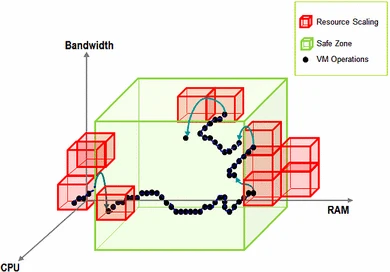
\includegraphics[scale=1.2]{img/SDTScaling.png}
  \caption{Safe-Zone and Resource Scaling Thresholds (from Paper ACCRS: autonomic based cloud computing resource scaling )}
\end{figure}

Die Grafik stellt die Safe-Zone als grünen Bereich, die Over- bzw. Under-Utilization als rote Würfel, die an die Grenzen der Safe-Zone grenzen, dar. Die X,Y und Z-Achsen repräsentieren die Auslastung von RAM, Netzwerk und CPU. Anhand von Sprüngen, die der Graph der VM-Operations nach überschreiten der Safe-Zone Grenze zurück in die Safe-Zone macht, kann nachvollzogen werden, dass skaliert wurde und so die Last pro VM gesunken ist.

Die Skalierung in diesem Projekt orientiert sich an dem Verfahren, welches im Paper \glqq ACCRS: autonomic based cloud computing resource scaling\grqq \cite{AlSharif.2016} eingesetzt wird. Die Idee der Zustände Safe-Zone, Under-Utilization sowie Over-Utilization und deren Erkennung mittels statischer Regeln werden adaptiert und auf das Kubernetes-Konzept der Deployment-Skalierung übertragen, die Thresholds werden allerdings abgewandelt. 


\pagebreak
\section{Datenaggregation}

Die Datenaggregation, also das Erheben und Sammeln von Daten, ist zentraler Bestandteil des Projektes und der erste grundlegende Schritt. Das Ziel der Aggregation ist es, Daten (sog. Metriken) über den Zustand eines Kubernetes-Clusters (siehe Kapitel Grundlagen/Kubernetes) zu erhalten. Kubernetes stellt selbst Metriken zur Verfügung. Im Folgenden wird beschrieben wie diese Daten ausgelesen und für die weitere Verwendung aufbereitet werden.

\subsection{Datenquellen}

Als Datenquelle dienen potenziell alle Ziele, die von Prometheus mittels der Target-Discovery innerhalb des Kubernetes-Cluster gefunden werden und Daten bereitstellen.\\
Von besonderem Interesse für dieses Projekt sind hierbei alle system- und hardwarenahen Targets, wie der kubelet (siehe Kapitel Grundlagen) und cAdvisor in Pods und Containern.
Prinzipiell eignen sich alle Pods als Datenquelle, Container die produktive Services bereitstellen weisen hierbei ein erhöhtes Interesse auf, gleiches gilt ebenso für produktiv betriebene Nodes.

\subsubsection{\glqq USE\grqq-Methode}

Das Monitoring der Systemressourcen wird nach der \glqq USE\grqq-Methode durchgeführt. Diese Methode wurde von Brendan Gregg, einem Netflix-Ingenieur im Bereich Cloud-Performance, mit Schwerpunkt auf das Monitoring von Systemressourcen entwickelt, weshalb sie sich für dieses Projekt eignet.
Ziel der Methode ist es, die Utilization, Saturation und Error-Rate von Systemkomponenten abzubilden. Die Utilization ist der Zeitdurchschnitt der Arbeit, die eine Ressource beschäftigt ist. Die Saturation, die \glqq Zusatzarbeit\grqq die eine Ressource verrichten muss, im Moment aber nicht leisten kann. Die Error-Rate ist die Häufigkeit in der Fehler bei einer Ressource auftreten.\\
Systemressource, die es sich lohnt zu überwachen, sind unter anderem:\\

\begin{itemize}
\item CPUs: Sockets, Kerne, Hardware-Threads (virtuelle CPUs)
\item RAM: Kapazität
\item Netzwerkinterfaces
\item Speicher(Festplatte,SSD): I/O, Kapazität
\item Controller: Storage, Netzwerkkarten
\end{itemize}

Laut Gregg ist die Methode für Geräte besonders sinnvoll und effektiv, die bei erhöhter Utilization oder Saturation einen Performanceeinbruch erleiden.\\

Gregg will mit dieser Methode eine Möglichkeit bieten, serverseitige Performanceprobleme schnell zu erkennen, deren Ursache zu finden, um diese dann eliminieren zu können. Sein Ziel ist es mit dieser Methode eine einfache und unkomplizierte, aber trotzdem schnelle und komplette Methode zu liefern. Laut Gregg hat sich diese Methode schon in vielen Bereichen mehrfach bewährt. In verschiedenen Unternehmen, als Lehrmittel in Schulklassen oder vor Allem aktuell im Cloud-Computing Bereich wird sie verwendet.\\

\begin{figure}[htbp]
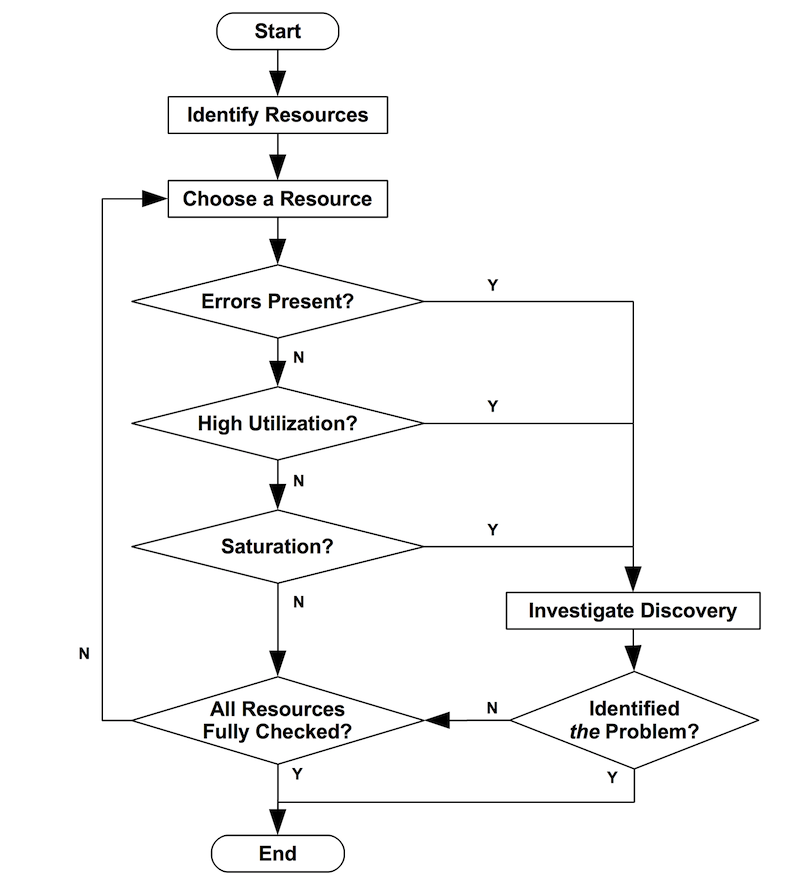
\includegraphics[scale=.7]{img/usemethod_flow.png}
\caption{Darstellung der Vorgehensweise bei Anwendung der USE-Methode ~\protect\cite{.20200810T18:06:18.000Z}}
\end{figure}

Die Reihenfolge des Vorgehens wird in diesem Diagram dargestellt. Um die Geschwindigkeit zu optimieren sollten Errors als erstes überprüft werden, da sie typischerweise schneller und einfacher zu interpretieren sind. Die Utilization oder Saturation können in beliebiger Reihenfolge beobachtet werden.
\cite{.27.07.2020}

\pagebreak

\subsubsection{Metriken}

Die Metriken, mit denen die USE-Methode umgesetzt wird, werden aus den Systemmetriken, die durch Prometheus gesammelt werden, zusammengesetzt. 
Die Metriken Utilization und Saturation werden für CPU, RAM und Netzwerkauslastung folgendermaßen berechnet:

\begin{description}
\item[CPU]:\\
\underline{Utilization:}\\
Die CPU Utilization berechnet sich aus der Summe der Millisekunden, welche die CPU beschäftigt war, geteilt durch eine ganze Sekunde. So erhält man die Utilization pro Sekunde, welche aufsummiert und der Mittelwert über den beobachteten Zeitraum gebildet wird, um so die durchschnittliche Utilization zu erhalten.\\

Der gleitende Mittelwert der aufsummierten Zeit U über den beobachteten Zeitraum von 5 Minuten:\\
Imax entspricht 300 Sekunden

\begin{minipage}{\linewidth}
\(
\displaystyle{U_{CPU}(t)=\frac{1}{N}{\sum\limits_{i_{w}=0}^{N-1} l_{cpu}{(t-i_{w})}} }
\)

\captionof{figure}{Formel der CPU-Utilization} 

\end{minipage}

Der gesamte Wert eines Utilization Fensters lässt sich dann über die zusammengesetzte Formel berechnen:\\

\underline{Saturation:}\\
Die CPU Saturation kann anhand des Ressourcenlimits berechnet werden. In UNIX basierten Betriebssystemen gibt es die Metrik \glqq load\_average\grqq, welche die Anzahl der laufenden sowie wartenden Prozesse enthält. Sofern man diese durch die Anzahl der zur Verfügung stehenden CPU-Kerne \glqq core\_unit\_count\grqq teilt, erhält man eine Kennzahl für die Saturation.\\

\begin{minipage}{\linewidth}
\(
\displaystyle{s_{cpu}= load\_average / core\_unit\_count}
\)
\captionof{figure}{Formel der CPU-Saturation} 

\end{minipage}\\

Diese aufsummiert und über die Zeit gemittelt, ergibt die durchschnittliche Saturation.\\

\begin{minipage}{\linewidth}
\(
\displaystyle{S_{CPU}(t)=\frac{1}{N}{\sum\limits_{i_{w}=0}^{N-1} s_{cpu}{(t-i_{w})}} }
\)
\captionof{figure}{Formel der CPU-Saturation Moving-Average} 

\end{minipage}

Ein weiterer Weg die Saturation zu berechnen, ist das Aufsummieren der Zeit in der ein Prozess \glqq throtteld\grqq läuft. Dies funktioniert dann, wenn ein Prozess ein Ressourcenlimit besitzt. Übersteigt er dieses, wird der Prozess gedrosselt.\\
\underline{Error-Rate:}\\
Die Fehlererkennung wird von handelsüblichen CPUs nicht unterstützt, weswegen in den meisten Fällen keine Fehlererkennung umgesetzt werden kann. Eine mögliche Fehlererkennung würde beispielsweise über ein sogenanntes Lockstep-Verfahren umgesetzt werden, bei dem zwei CPUs jeweils die gleiche Aufgabe erhalten und gegenseitig ihre Ergebnisse vergleichen. Bei Unterschieden im Ergebnis kann daraus ein Fehlerfall ermittelt werden\cite{.}<Zitat US-Patent>.
\item[RAM]:\\
\underline{Utilization:}\\
Die RAM Utilization berechnet sich aus der Menge des vom System reservierten Speichers, der durch die Menge des gesamten Speichers geteilt wird. Beide stehen in UNIX basierten Betriebssystemen zur Verfügung, sodass die Rechnung zur RAM-Utilization lautet:\\

\begin{minipage}{\linewidth}
\(
\displaystyle{l_{ram}=1-ram_{res}/ram_{ges}}
\) 
\captionof{figure}{Formel der RAM-Utilization} 

\end{minipage}

Diese aufsummiert und über die Zeit gemittelt, ergibt die durchschnittliche Utilization.\\

\begin{minipage}{\linewidth}
\(
\displaystyle{U_{RAM}(t)=\frac{1}{N}{\sum\limits_{i_{w}=0}^{N-1} l_{ram}{(t-i_{w})}} }
\) 
\\
\captionof{figure}{Formel der RAM-Utilization Moving-Average} 
\end{minipage}

\pagebreak

\underline{Saturation:}\\
Die RAM Saturation kann am besten berechnet werden, wenn Ressourcenlimits existieren. Unter diesen Voraussetzungen kann die Saturation berechnet werden, indem die Summe des aktuell verwendeten Speichers durch das Ressourcenlimit geteilt wird. Sofern ein Wert über 100\% erreicht wird\\

\begin{minipage}{\linewidth}
\(
\displaystyle{s_{ram}=RAM_{res}/RAM_{ges}}
\) 
\captionof{figure}{Formel der RAM-Saturation} 
\end{minipage}

Über diesen wird wiederum der Mittelwert gebildet:\\

\begin{minipage}{\linewidth}
\(
\displaystyle{S_{RAM}(t)=\frac{1}{N}{\sum\limits_{i_{w}=0}^{N-1} s_{ram}{(t-i_{w})}} }
\) 
\captionof{figure}{Formel der RAM-Saturation Moving-Average} 
\end{minipage}

\underline{Error-Rate:}\\
Zur Ermittlung von Fehlern im Arbeitsspeicher wird sogenanntes \glqq Error Correcting Code\grqq(ECC)-RAM benötigt. Dieses RAM erkennt Fehler in Speicherzellen des Arbeitsspeichers, die aufsummiert die Fehlerrate des RAMs ergeben. Sofern dieses RAM nicht eingesetzt wird ist eine Fehlerkennung nicht genau möglich. Ein alternatives aber möglicherweise ungenaueres Verfahren wäre das Feststellen von fehlgeschlagenen Speicherreservierungen. Dieses Verfahren zählt jedoch Fehlschläge des virtuellen Speicher und nicht des phyischen, was zu Messungenauigkeiten führen kann.
Die Berechnung der Fehlerrate wäre wie folgt:\\

\begin{minipage}{\linewidth}
\(
\displaystyle{E_{RAM}(t)=\frac{1}{N}{\sum\limits_{i_{w}=0}^{N-1} e_{ram}{(t-i_{w})}} }
\) 
\captionof{figure}{Formel der RAM-Error-Rate} 
\end{minipage}

\pagebreak

\item[Netzwerk-Bandbreite]:\\
\underline{Utilization:}\\
Um die Netzwerk Utilization zu messen, werden die Bytes aufsummiert, die versendet sowie empfangen werden und daraus der Mittelwert berechnet.\\

\begin{minipage}{\linewidth}
\(
\displaystyle{U_{Net}(t)=\frac{1}{N}{\sum\limits_{i_{w}=0}^{N-1} l_{net}{(t-i_{w})}} }
\) 
\captionof{figure}{Formel der Netzwerk-Utilization} 
\end{minipage}

\underline{Saturation:}\\
Die Netzwerk Saturation kann nur dann sinnvoll gemessen werden, wenn das Bandbreitenlimit bekannt ist. Sofern dies der Fall ist kann die Saturation berechnet werden, indem die versendeten bzw. empfangenen Bytes(u\_bytes) durch das Bandbreitenlimit geteilt wird. \\

\begin{minipage}{\linewidth}
\(
\displaystyle{s_{net}=u\_bytes/bandwidth}
\) 
\captionof{figure}{Formel der Netzwerk-Saturation} 
\end{minipage}

Über diese wird wiederum der Mittelwert gebildet.

\begin{minipage}{\linewidth}
\(
\displaystyle{S_{Net}(t)=\frac{1}{N}{\sum\limits_{i_{w}=0}^{N-1} s_{net}{(t-i_{w})}} }
\) 
\captionof{figure}{Formel der Netzwerk-Saturation Moving-Average} 
\end{minipage}

Sofern keine Information zum Limit zur Verfügung stehen, können die verworfenen Pakete (dropped Packages) als Indikator dafür dienen, wie hoch die Saturation ist.\\

\underline{Error-Rate:}\\
Zum Ermitteln der Error-Rate des Netzwerks werden Sende- und Empfangs-Fehler aufsummiert, welche die Error-Rate bilden.

\begin{minipage}{\linewidth}
\(
\displaystyle{E_{Net}(t)=\frac{1}{N}{\sum\limits_{i_{w}=0}^{N-1} e_{net}{(t-i_{w})}} }
\) 
\captionof{figure}{Formel der Netzwerk-Error-Rate} 
\end{minipage}

\end{description}
\subsection{Tools}
\subsubsection{Datenaggregation}

Das Monitoringtool, welches in diesem Projekt zur Datenaggregation genutzt wird, ist Prometheus. Aufgrund seines Status als Quasi-Standard im Cloud-Native Umfeld und für das Monitoring von Kubernetes wird Prometheus in diesem Projekt verwendet, da es neben hohen Kompatibilität zu anderen Systemen auch eine sehr gute Dokumentation aufweist. Für dieses Projekt bietet es zentrale Features, welche die Umsetzung ermöglichen.

Wichtige Features von Prometheus zur Datenaggregation sind:
\begin{description}

\item[Automatische Service-Discovery]
Das Feature der automatischen Service-Discovery ist sehr entscheidend, da sich die Services im Cluster häufig verändern und neue Services hinzugefügt werden. Mithilfe dieser Funktion werden Services automatisch gefunden, Metriken direkt erhoben und Regeln auf diese angewendet, ohne konfiguriert werden zu müssen.
\item[Echtzeitmetriken]
Prometheus zeichnet Metriken in Echtzeit auf. Das ermöglicht es, jederzeit den aktuellen Status des Clusters einzusehen und in Echtzeit darauf reagieren zu können.
\item[Zeitreihen]
Prometheus zeichnet Metriken als Zeitreihen auf, was das Beobachten, Abfragen und die Definition von Regeln über Zeiträume ermöglicht. 

\end{description}


Neben den Features zur Datenaggregation bietet Prometheus auch noch weitere für dieses Projekt wichtige Features :
\begin{description}
\item[Regeln]
Regeln spielen eine zentrale Rolle in diesem Projekt. Mithilfe dieser lassen sich verschiedene Features von Prometheus regulieren. In diesem Projekt werden sie für das Regulieren von Alerts verwendet.
Regeln werden über Thresholds und optional über Zeiträume von Metriken definiert, sodass bei Überschreiten eines Thresholds für eine bestimmte Zeit eine Regel als erfült gilt.
\item[Alerting]
Mithilfe der Alerts ist es möglich, anhand von Regeln Alarme zu versenden, die über den Zustand des Clusters informieren. Sie können an Ziele wie E-Mail-Adressen oder Chat-Tools wie Slack oder Telegram gesendet werden, aber auch  an selbst definierte Endpunkte, um sie dort zu empfangen oder sie möglicherweise weiterzuverarbeiten.

\end{description}
\pagebreak
\newpage
\subsubsection{Ablauf der Aggregation}

Die Aggregation der Metriken läuft nach festen Schema ab, welches für die Aufzeichnung aller Metriken gilt.
Die Metriken werden von Prometheus aggregiert und aufgezeichnet. Dies wird auf allen Zielen, welche durch die automatische Service-Discovery gefunden wurden durchgeführt.\\

\begin{figure}[htbp]
\begin{minipage}[t]{6cm}
\vspace{0pt}
Die Metriken werden über einen definierten Zeitraum gesammelt, sodass daraus Zeitreihen-Metriken entstehen. Aus diesen Zeitreihenmetriken kann ein Graf abgeleitet werden.\\
\end{minipage}
\hfill
\begin{minipage}[t]{6cm}
\vspace{0pt}
\centering
  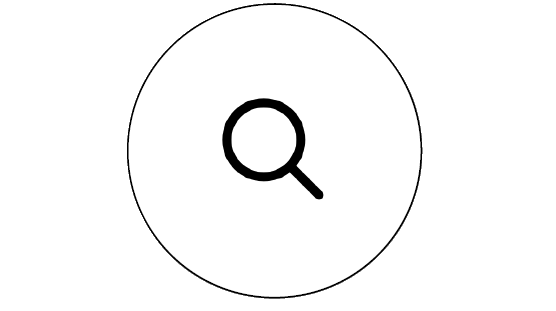
\includegraphics[scale=.3]{img/Datenaggregation/LupeNew.png} 
\caption{Bildrepräsentation des Alarms (Quelle Draw.io)}
\label{fig:Bild1}
\end{minipage}
\end{figure}

\begin{figure}[htbp]
\begin{minipage}[t]{6cm}
\vspace{0pt}
Wenn man diese Zeitreihenmetriken in ein Koordinatensystem überträgt, wäre die X-Achse eines Grafen der Zeitwert zwischen Null und maximalem aufgezeichnetem Zeitwert und die Y-Achse die höhe des Metrikwertes. \\
\end{minipage}
\hfill
\begin{minipage}[t]{6cm}
\vspace{0pt}
\centering
  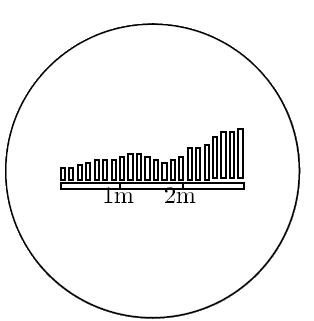
\includegraphics[scale=.3]{img/Datenaggregation/GrafAggregationNew.png}
\caption{Bildrepräsentation der Zeitreihe}
\label{fig:Bild1}
\end{minipage}
\end{figure}

\begin{figure}[htbp]
\begin{minipage}[t]{6cm}
\vspace{0pt}
Anhand der Höhe des Y-Wertes des Grafen lassen sich Regeln definieren und somit ein Grenzwert für Metriken erstellen.\\
\end{minipage}
\hfill
\begin{minipage}[t]{6cm}
\vspace{0pt}
\centering
  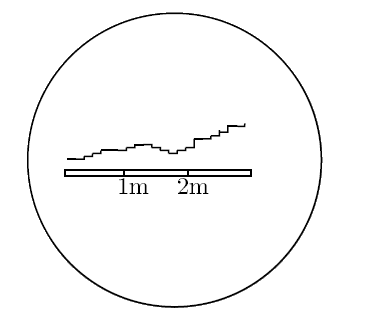
\includegraphics[scale=.3]{img/Datenaggregation/GrafZeitNew.png}
\caption{Bildrepräsentation der Zeitreihe als Graf}
\label{fig:Bild1}
\end{minipage}
\end{figure}

\begin{figure}[htbp]
\begin{minipage}[t]{6cm}
\vspace{0pt}
Über den Zeitwert (X-Achse) wird eine Dauer definiert, die der Zustand der Grenzwertüberschreitung bestehen darf.\\
\end{minipage}
\hfill
\begin{minipage}[t]{6cm}
\vspace{0pt}
\centering
  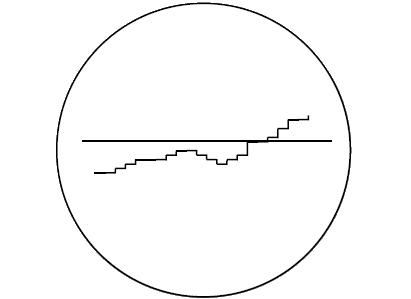
\includegraphics[scale=.3]{img/Datenaggregation/GrafYWertNew.png} 
\caption{Bild1}
\label{fig:Bild1}
\end{minipage}
\end{figure}

\begin{figure}[htbp]
\begin{minipage}[t]{6cm}
\vspace{0pt}
Wenn der Grenzwert über die definierte Zeitdauer überschritten wurde wird ein Alarm ausgelöst.\\
\end{minipage}
\hfill
\begin{minipage}[t]{6cm}
\vspace{0pt}
\centering
  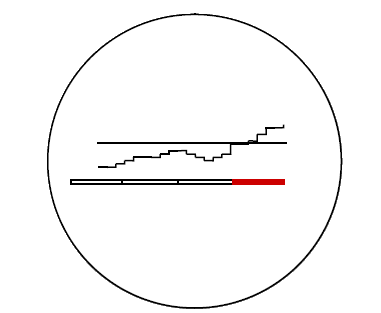
\includegraphics[scale=.3]{img/Datenaggregation/GrafAlarmNew.png} 
\caption{Bildrepräsentation des Graf mit Y-Achsen Grenzwert}
\label{fig:Bild1}
\end{minipage}
\end{figure}

\begin{figure}[htbp]
\begin{minipage}[t]{6cm}
\vspace{0pt}
Wenn der Grenzwert über die definierte Zeitdauer überschritten wurde wird ein Alarm ausgelöst.\\
Im nachfolgenden Graf wird der Ablauf der Aggregation aufeinander aufbauend visualisiert:
\end{minipage}
\hfill
\begin{minipage}[t]{6cm}
\vspace{0pt}
\centering
  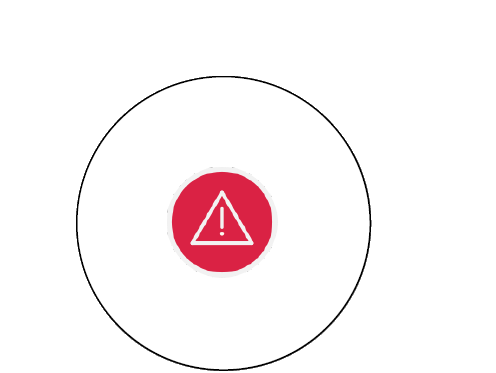
\includegraphics[scale=.3]{img/Datenaggregation/AlarmNew.png}  
\caption{Bildrepräsentation des Alarms(Quelle Draw.io)}
\label{fig:Bild1}
\end{minipage}
\end{figure}



\begin{minipage}{\linewidth}
  \centering
  \scalebox{.8}{\input{DatenaggregationFlow.pdf_tex}} 
  \captionof{figure}{Graf des Ablaufs der Datenaggregation}
\end{minipage}



\subsubsection{Visualisierung}

Grafana ist das Tool, welches zur Visualisierung verwendet wird. Das Open-Source Tool bietet Möglichkeiten, Metriken in Form von Graphen, Zählern, Histogrammen und vielem mehr über Zeiträume zu visualisieren. Des Weiteren können ganze \glqq Dashboards\grqq erstellt werden, die den Überblick über das ganze Cluster auf einmal erlauben.\\
Aufgrund der bereits vorhandenen Prometheusintegration ist eine Verwendung bei bereits bestehendem Prometheus-Server einfach und innerhalb kurzer Zeit umzusetzen.
Der Prometheus-Server, von welchem Grafana Metriken erhalten soll muss als Datenquelle mittels seiner Adresse konfiguriert werden. Danach stehen alle Metriken, welche Prometheus kennt auch in Grafana zur Verfügung.\\
Um Metriken zu visualisieren, wird die aus Prometheus bereits bekannte Abfragesprache PromQL verwendet, was den Vorteil bietet, Abfragen, die für Prometheus funktionieren, ebenfalls in der Grafana Oberfläche zum Erstellen von Visualisierungen zu verwenden.\\
Da Grafana eines der gängistens Tools ist und teilweise als Quasi-Standard zur Visualisierung von Metriken behandelt wird, findet eine kontinuierliche Weiterentwicklung statt und eine große Community bietet Unterstützung und Erfahrungen.\\%<hier Quelle Logz.io einfügen>

\section{Auswerten der Metriken}

Das Auswerten der Metriken erfolgt für das Monitoring durch das Umsetzen der USE-Methode (beschrieben in Kapitel vier).

\subsection{Klassifizierung}

Die Metriken werden in Node-Level sowie Pod-Level Metriken klassifiziert.\\
Nodelevelmetriken repräsentieren den Zustand eines ganzen Nodes, das bedeutet, dass die Metriken die Summe aller Pods, Container, Services, etc. des Nodes darstellen.\\
Podlevelmetriken hingegen repräsentieren den Status eines einzelnen Pods.\\
Die Podlevelmetriken werden visualisiert um Zustände einzelner Pods einsehen zu können, finden aber vor allem auch bei der Automatisierung von Aktionen ihren Nutzen. Für diese Metriken werden Regeln erstellt, die zur automatisierten Anwendung von Aktionen auf einen Pod dienen.\\
Nodelevelmetriken werden in diesem Projekt vor allem zum Überwachen des Zustandes des gesamten Nodes verwendet und dienen dazu, kritische Zustände eines ganzen Nodes zu erkennen. Daher werden diese visualiert, finden aber bei der Automatisierung und dem Alerting keine weitere Verwendung.

\subsection{Logische Auswertung}

Die logische Auswertung der Metriken findet an zwei Stellen in diesem Projekt Anwendung. Einmal zum Erstellen von Alerting-Regeln auf dem Prometheus-Server und einmal zur grafischen Darstellung der Metriken in der Grafana-Oberfläche. In beiden Fällen wird zur Auswertung die PromQL-Sprache verwendet.
Zur logischen Auswertung werden die von Prometheus aggregierten Daten verwendet. Für das Monitoring werden die Schritte der USE-Methode Utilization, Saturation und Error-Rate jeweils für CPU, RAM sowie Netzwerk umgesetzt (siehe Kapitel vier,Metriken). Diese Metriken werden mittels eines \glqq Moving Average\grqq-Filters mit einer Fensterbreite von fünf Minuten gefiltert und ausgewertet. Dies hat zur Folge, dass Ausreißer in der Last nicht schwer ins Gewicht fallen und so starke Schwankungen verhindert werden, was zur Verbesserung der Beobachtbarkeit beiträgt.\\
Der eingesetzte \glqq Moving-Average\grqq-Filter sieht folgendermaßen aus:\\

\begin{Huge}

\(
\displaystyle{m^{(n)}_{MA}(t) = \frac{1}{n}{\sum\limits_{i=0}^{{n-1}} x_{(t-i)}} }
\)\\
\captionof{figure}{Formel des \glqq Moving-Average\grqq-Filter}

\end{Huge}

Der Zeitraum von fünf Minuten wurde so gewählt, da bei einem längerem Zeitraum, von beispielsweise zehn Minuten, die beobachtete Menge an Metriken größer wird und so die Reaktionszeiten auf Leistungsschwankungen durch langsamer ansteigende Mittelwerte länger werden.
Der umgekehrte Fall tritt ein, wenn ein zu kurzer Zeitraum gewählt wird, hierdurch werden Mittelwertschwankungen möglicherweise überbewertet wodurch Ausreißer eine zu große Bedeutung einnehmen.
Der gewählte Wert von fünf Minuten ist ein variabler Wert, der je nach Lastprofil auch angepasst und verändert werden kann.

\subsection{Metric-to-Action Methode}

Für die logische Auswertung der Daten werden neben dem reinen Auslesen von Metriken auch Grenzwerte benötigt. Zu diesem Zweck ist in diesem Projekt die \glqq Metric-to-Action\grqq-Methode entwickelt worden, welche die Ansätze der USE-Methode mit Grenzwerten verknüpft.\\
Diese Methode verwendet die Utilization-Metriken von USE, in diesem Projekt, zu CPU, RAM und Netzwerklast, welche mit Grenzwerten vereint werden.\\
Das Ziel ist es über ein beliebiges Zeitfenster Metriken anhand von Grenzwerten zu beobachten, die zusammen einen binären Wert ergeben. Die Methode ist dann sinnvoll, wenn anhand von Metriken regelbasiert entschieden werden soll, wie auf diese reagiert werden kann.

\subsection{Graphische Aufbereitung}

Zur Visualisierung der Metriken stehen in der Grafana-Oberfläche verschiedene Möglichkeiten zur Verfügung. Da es das Ziel ist möglichst auf einen Blick, den Systemressourcenzustand des ganzen Clusters sehen zu können, wird ein Dashboard mit allen USE-Metriken erstellt. Die Metriken können als Graph, Zähler, Balkendiagramm oder Heat-Map dargestellt werden.\\
Da schnell erkennbar sein soll, an welcher Stelle ungewöhnliche oder kritische Werte auftreten, werden die Zähler als Visualisierungsmethode für alle Metriken gewählt. Hierbei steht pro Metrik ein eigener Zähler zur Verfügung, womit sich der Zustand jeder Ressource einzeln einsehen lässt.\\
Für die Counter werden grüne Bereiche für unkritische Auslastung und rote Bereiche für kritische Auslastung mit einen Grenzwert von 75\% eingerichtet, um kritische Zustände hervorzuheben.

\begin{figure}[htbp]
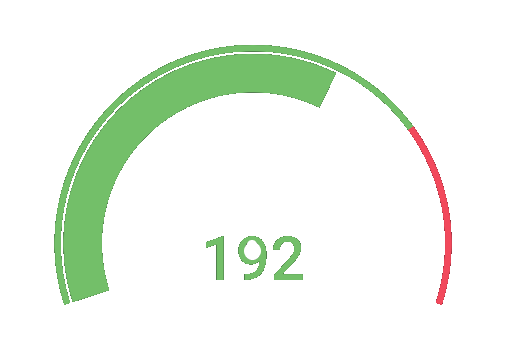
\includegraphics[scale=.8]{img/PercantageTransparent.png}
\caption{Darstellung des Counters}
\end{figure}


\section{Automatisierte Aktionen}

Das Kernthema dieser Arbeit ist die Entwicklung eines Systems, welches das Ausführen automatisierter Aktionen auf ein Kubernetes-Cluster ermöglicht. Mithilfe der Komponenten und Tools, Prometheus und dessen Alert-Verwaltungstool \glqq Alertmanager\grqq (siehe Grundlagenkapitel) sowie einer Eigenentwicklung, genannt \glqq Alert-Action-Manager\grqq, welcher Alerts empfängt und auf diese mit einer passenden automatisierten Aktion reagiert, wird dieses Vorhaben in diesem Kapitel umgesetzt. Mittels automatischer Skalierung und Anomalie-Detection wird die Funktion der Systems und der Komponenten nachgewiesen.


\pagebreak
\subsection{Architektur des Systems}

Das System, welches die automatisierten Aktionen möglich macht, besteht aus mehreren, voneinander abhängigen Komponenten. Das Konzept nutzt das Alerting-Feature von Prometheus und setzt mithilfe dessen automatisierte Aktionen um.\\

\begin{figure}[htbp]
  \centering
  \scalebox{.6}{\input{Architektur.pdf_tex}}
  \caption{Aufbau der Architektur}
\end{figure}

Die Architektur, welche in diesem Projekt entwickelt wurde, besteht aus sechs Komponenten. Vier davon, (Grafana, Prometheus Server und Alertmanager sowie der Alert-Action-Manager) wurden im Laufe des Projekts erstellt sowie konfiguriert bzw. entwickelt. Zwei davon, das Kubernetes-Cluster, auf dem dieses Projekt basiert, sowie Slack, bestanden schon vorher und wurden in das Projekt miteinbezogen. Die vier für Komponenten Grafana, Prometheus Server und Alertmanager sowie der Alert-Action-Manager laufen selbst als Deployment im Kubernetes-Cluster.\\
Im Folgenden wird die Architektur nach Bestandteilen erklärt:\\
\begin{description}
\item[Kubernetes-Cluster:]
Das Kubernetes-Cluster, auf dem Webservices sowie andere Backendsoftware laufen, ist das Ziel des Monitorings sowie der automatisierten Aktionen. Kubernetes stellt Metriken von sich aus bereit, welche ausgelesen und verarbeitet werden. Die Architektur läuft losgelöst vom restlichen Cluster und dessen Software, sodass durch dieses Projekt keine zusätzliche Anpassung oder Konfiguration von bestehender Software benötigt wird.
\item[Prometheus-Server:]
Der Prometheus-Server bildet das Herzstück der Architektur. Er aggregiert die durch das Kubernetes-Cluster bereitgestellten Metriken und wendet Regeln, wie das Alerting, auf diese an. Außerdem macht er diese Metriken, entweder durch das eigene Web-UI oder durch weitere Tools, mittels der Abfragesprache PromQL wieder abrufbar.
\item[Grafana:]
Grafana ist das in dieser Architektur eingesetzte Visualisierungstool, mit dem Administrator und andere Benutzer den Zustand des Clusters graphisch aufbereitet einsehen können. Das Tool bietet gegenüber der nativen Prometheus Web-UI deutlich bessere Darstellungsmöglichkeiten (siehe hierzu Kapitel Auswertung der Metriken). Grafana ruft Metriken direkt vom Prometheus-Server ab und unterstützt auch dessen Query-Language PromQL.
\item[Prometheus-Alertmanager:]
Der Prometheus-Alertmanager empfängt Alerts direkt durch den Prometheus-Server. Seine Aufgabe ist es, empfangene Alerts an seine Ziele \glqq Alert-Action-Manager\grqq sowie \glqq Slack\grqq und darauf eingerichteten Alert-Channel weiterzuverteilen.
\item[Alert-Action-Manager:]
Der \glqq Alert-Action-Manager\grqq empfängt Nachrichten durch den Prometheus-Alertmanager. Dieses Tool ist eine komplette Eigenentwicklung und dafür zuständig, dass auf empfange Alerts mit entsprechenden Aktionen auf das Kubernetes-Cluster reagiert wird.
\item[Slack:]
Slack ist die Benachrichtigungsplattform für Administratoren und interessierte Benutzer. Hier wurde ein eigener Channel für den Zweck der Benachrichtigung beim Auftreten von Alerts eingerichtet.

\end{description}

Auf wichtige Komponenten wird hier nochmal gesondert eingegangen.

\subsubsection{Prometheus}

Wie bereits beschrieben, bildet Prometheus die zentrale Komponente in diesem Projekt und dessen Architektur. Auf dem Prometheus-Server werden alle Regeln definiert und konfiguriert, die für das Alerting benötigt werden und damit Aktionen auslösen können. Außerdem können auf dem Server die Zeiten konfiguriert werden, in deren Abständen der Server Metriken scraped, Regeln prüft und Alerts sendet. Diese Zeiten bestimmen maßgeblich in welcher Geschwindigkeit die Aktionen ausgeführt werden und können verhindern, dass Alert-Nachrichten zu häufig und in zu kurzen Abständen versendet werden.\\

Zusätzlich zum zentralen Server besitzt Prometheus auch Komponenten, die direkt im Kubernetes-Cluster auf den Nodes laufen und dafür sorgen, dass von Kubernetes mittels kubelet und cAdvisor (siehe Kapitel Grundlagen/Kubernetes) veröffentlichte Metriken für den Server bereitgestellt werden. Diese Aufgabe übernehmen die Exporter, welche im Cluster installiert und konfiguriert sind.
Der Prometheus-Server, wie auch der Alertmanager, stellen ein eigenes Deployment dar und laufen als Pod im Kubernetes-Cluster. 

\subsubsection{Alertmanager}

Der Prometheus-Alertmanager, der in der Architektur als Message-Broker von Alerts dient, ermöglicht die grundsätzliche Kommunikation zwischen Prometheus und externen Tools. Die Möglichkeit, mittels des Nachrichtensystems neben vorkonfigurierten Drittanbietertools wie Slack auch eigene sog. Webhooks zu adressieren, erlaubt die Möglichkeit einen eigenen HTTP-Endpunkt als Nachrichtenziel zu verwenden. Da sich für einen Alert mehrere Ziele festlegen lassen, kann so zu jeder automatischen Aktion auch eine Warnung an den für Alerts konfigurierten Slack-Channel gesendet werden. So kann in zukünftigen Alerts auch zwischen rein informativem Alert, der nur an Slack gesendet wird, und einem Alert, der eine Aktion zur Folge hat, unterschieden werden und diese entsprechend konfiguriert, werden.\\

\subsubsection{Regeln}

Die Regeln, die zum Aktivieren der Alerts verwendet werden, bestehen aus einem Label, einem Ausdruck, der Metriken abgleicht und einem Erfüllungszeitrahmen.
Der Ausdruck ist, wie die Queries zur Visualisierung auch, in der PromQL-Sprache geschrieben. Ein Ausdruck muss immer als Vergleich geschrieben werden und somit einen boolschen Wert repräsentieren können, also erfüllt (true) oder nicht erfüllt (false).
Jeder Ausdruck besitzt einen Zeitrahmen über den er erfüllt sein muss um einen Alert auszulösen, womit vorzeitiges oder zu häufiges Alarmieren eingeschränkt oder verhindert werden kann.
Um mehrere Bedingungen in einem Ausdruck zu verknüpfen, kann auf logische Operatoren zurückgegriffen werden. Diese sind AND, OR und UNLESS (Komplement).
Zum Inkludieren oder Exkludieren einzelner Metrikquellen, können mittels der Anwendung von regulären Ausdrücken auf die Namen der Quellen Filter für diese erstellt werden.

Die grobe Struktur eines Alerts sieht folgerndermaßen aus:\\

\begin{lstlisting}[basicstyle=\footnotesize]
     Label:		"Musterlabel"
     Regel:		a > b
     Offsetzeit:	5 Minuten
     Anmerkungen:	In Musterlabel ist a kleiner b
\end{lstlisting}

Ein Alert muss identifiziert werden können. Hierfür wird das Label verwendet, das den Namen eindeutig repräsentiert.\\
Alerts sollen nur dann ausgelöst werden, wenn ein entsprechender Zustand erfüllt ist. Um diesen Zustand zu spezifizieren wird die Vergleichsregel zum Bemessen gebraucht.\\
Um kurzzeitige Ausreißer im Zustand nicht überzubewerten, muss dieser eine gewisse Dauer vorliegen. Diese Dauer, auch Offsetzeit genannt, wird zusätzlich zur Regel spezifiziert.\\
Je nach Alert oder auszuführender Aktion werden Zusatzinformationen benötigt. Diese können als Anmerkung beigefügt werden. Unter anderem kann hier beschrieben werden, wie eine Alert-Nachricht als Chatnachricht aussehen soll.\\

Der Ablauf des Konzepts ist eine Kette von Aktionen, bei der ein Schritt den nächsten auslöst. Die Kette der Schritte, welche zum Auslösen und Ausführen einer Aktion durchlaufen wird, ist hier beschrieben:\\

\pagebreak

\begin{wrapfigure}{r}{0.5\textwidth}

\begin{center}
  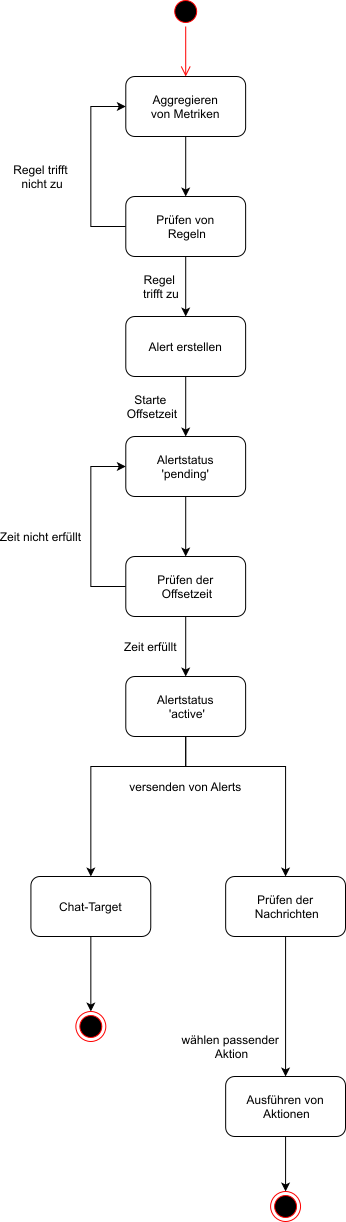
\includegraphics[width=0.42\textwidth,height=1.32\textwidth]{img/AAMtextless.PNG}
  \caption{Ablaufgraph}
\end{center}

\end{wrapfigure}
\textbf{Schritt 1:}\\
Im ersten Schritt aggregiert der Prometheus-Server
aus dem Kubernetes-Cluster Systemressourcen bezogene Metriken
von Pods und Containern.\\

\textbf{Schritt 2:}\\
In Schritt zwei prüft der Prometheus-Server anhand konfigurierter Alerting-Regeln,
ob ein Alert ausgelöst werden soll. Falls dies der Fall ist,
versendet der Server einen Alert an den Prometheus-Alertmanager,
 zuerst mit dem Status 'pending',
nach Ablauf der Offset-Zeit mit dem Status 'active' (siehe Kapitel Grundlagen/Alerting).

\textbf{Schritt 3:}\\
Der Alertmanager versendet, sobald ein Alert den Status 'active' erhält,
an alle konfigurierten Ziele eine Alert-Nachricht.
Diese sind ein Channel des Chatprogramms 'Slack',
der alleine für Alert-Nachrichten zur Verfügung steht und den Zweck
 besitzt Administratoren und andere Interessierte zu informieren,
sowie das in diesem Projekt entwickelte Tool 'Alert-Action-Manager',
welches den Zweck besitzt anhand eintreffender Alert-Nachrichten
 Aktionen auf das Kubernetes-Cluster auszuführen.\\
 
\textbf{Schritt 4:}\\
Beim Eintreffen von Alerts prüft der 'Alert-Action-Manager'
die eingehenden Nachrichten auf deren Inhalt
um festzustellen, welche Aktion ausgeführt werden soll.\\

\textbf{Schritt 5:}\\
Nachdem eine Nachricht durch den Alert-Action-Manager geprüft wurde,
wird eine entsprechende Aktion auf das Kubernetes-Cluster ausgeführt.\\

\section{Alert-Action-Manager}

Der Alert-Action-Manager (hier abgekürzt: AAM) ist eine eigenst entwickelte Komponente, um aus den von Prometheus versendeten Alerts automatisiert konkrete Aktionen zu schließen und auf das Kubernetes-Cluster anzuwenden.\\


\subsection{Anforderungen}

An den AAM sind mehrere Anforderungen geknüpft, die er erfüllen muss, um seine Aufgabe adäquat umsetzen zu können.

\begin{itemize}
\item von Prometheus versendete Alerts müssen empfangen werden können
\item der Manager muss mit dem gegebenen Format JSON umgehen können
\item ein fest konfigurierbarer HTTP-Endpunkt wird benötigt
\item der Manager muss  aus den gegebenen Informationen eines Alerts Aktionen schließen können
\item um Aktionen auf das Cluster ausführen zu können, muss der Manager eine Schnittstelle zu Kubernetes besitzen
\end{itemize}

\subsection{Funktionen}

Um die beschriebenen Anforderungen umzusetzen, besitzt der AAM diese grundlegenden Funktionen:\\

\begin{description}

\item[HTTP-Endpunkte:]
Für den AAM wird ein eigener Kubernetes-Service bereitgestellt, der als DNS-Service fungiert.
Um Alerts zu empfangen, wird ein HTTP-POST Endpunkt bereitgestellt. Der Prometheus-Alertmanager wird so konfiguriert, dass er Alerts an den Kubernetes-Service des AAM sendet. Die Requests werden im JSON-Format empfangen, welches auch das Standardformat ist, in dem die Alerts versendet werden.
Weitere Endpunkte sind der \glqq health\grqq Pfad, über den sich überprüfen lässt, ob der AAM erreichbar ist und der \glqq podstatus\grqq Pfad, über den sich der Podstatus des AAM und allen Pods in dessen Namespace, in dem sich alle Komponenten der Architektur befinden, einsehen und der korrekte Zugriff des Service auf das \glqq kubectl\grqq überprüfen lässt.
\item[Alert-Analyse:]
Alerts die über den HTTP-POST Endpunkt empfangen wurden, werden vom AAM analysiert und eingeordnet. Aus dem POST-Request wird zuerst das Label geparst, was die Einordnung des Alerts ermöglicht. Dieses wird mit den bekannten Labels verglichen. Falls es nicht bekannt ist, wird der Alert verworfen, sofern es bekannt ist, wird die Funktion des passenden Labels ausgeführt. Der erste Schritt einer Funktion ist das Analysieren des zugehörigen Deployments, also der Pod oder das Deployment auf welches eine Aktion ausgeführt werden soll. Hierzu wird der Name eines Pods verwendet oder vorher der Deployment-Name aus dem Namen des Pods geparst.
Nach erfolgreicher Analyse wird die passende Aktion ausgeführt.
\item[Ausführen von Aktionen:]
Das Ausführen von Aktionen wird mittels \glqq kubectl\grqq durchgeführt. Die erforderlichen Daten, die zum Durchführen einer kubectl-Aktion gebraucht werden, wurden vor dem Ausführen durch die Analyse ermittelt und nun in die Aktion eingebaut.
\item[Zusatzfunktionen:]
Es werden zum Ausführen einiger Aktionen zusätzliche Funktionen benötigt. Zum Skalieren der Replicas eines Deployments (beschrieben im folgenden Unterkapitel), ist die Anzahl der Replicas zum Zeitpunkt des Ausführens der Aktion erforderlich. Hierfür besitzt der AAM eine Funktion, welche die Replikaanzahl zu einem Deployment analysieren kann.

\end{description}

\subsection{Erweiterung}

Sofern zusätzliche Aktionen in der Infrastruktur benötigt werden, ist die Erweiterung mit relativ geringem Aufwand möglich. Es muss einerseits eine neue Regel bzw. neue Regeln mit neuem Label in Prometheus definiert werden sowie die zugehörige Aktion im AAM.

\subsection{Aktionen}

Die Aktionen, welche durch den Alert-Action-Manager automatisiert auf das Kubernetes-Cluster ausgeführt werden, sind in diesem Abschnitt erklärt. Das Ausführen dieser Aktionen wird anhand von Regeln mit statischen Grenzwerten sog. Thresholds entschieden.
Die beiden Aktionen, welche in diesem Projekt eingesetzt werden, sind die Skalierung der Pod-Replikationen eines Deployments und die Anomalie-Detection innerhalb eines Pods bzw. Containers.

\subsubsection{Skalierung}

Die Aktion der Skalierung ermöglicht das Hochskalieren, also das Erweitern eines Deployments um eine höhere Anzahl an Replikationen (Replicas) seiner Pods, sowie die Gegenaktion, das Herunterskalieren eines Deployments.\\
Diese Aktion wird durch zwei Regeln realisiert:

\begin{description}
\item[PodLowResource]

Diese Regel wird ausgelöst, sobald in einem Pod eine hohe Last der Ressourcen CPU-Utilization oder RAM-Utilization festgestellt wird und dies in Verbindung mit einer hohen Nutzerlast, also einer ausreichend hohen\\ Netzwerkbandbreiten-Utilization, steht. Die Thresholds für CPU- und RAM-Utilization liegen bei 75\%, die Auslastung der Netzwerkbandbreite muss bei mindestens einem Megabit pro Sekunde liegen. Diese Last muss für 10 Sekunden bestehen, um die \glqq PodLowResource\grqq -Regel und damit den Alert zu aktivieren.

\item[PodHighResource]

\glqq PodHighResource\grqq ist die Gegenaktion zu \glqq PodLowResource\grqq und wird dann ausgelöst, wenn 
eine niedrige Ressourcenlast in einem Deployment detektiert wird. Die geprüften Metriken sind die CPU-Utilization sowie die RAM-Utilization. Diese müssen über ein Zeitfenster von 10 Sekunden einen Wert von 25\% Auslastung oder niedriger aufweisen, um diese Regel zu erfüllen.

\end{description}

Nach Auslösen einer der Alerts und Aktivieren der Aktion im \glqq Alert-Action-Manager\grqq setzt dieser die Aktion folgendermaßen um:

Für diese Aktion wird einerseits der Name des Deployments benötigt sowie die Anzahl der Pod-Replikation, die zum Ausführungszeitpunkt der Regel existieren.\\
Der Name betroffener Pods wird mit einem Alert mitgeschickt. Durch entfernen des Pod-Tags kann daraus der Name des Deployments ermittelt werden.\\
Die Anzahl der Replikationen wird durch eine dafür bereitgestellte Methode aus dem Cluster ermittelt und zurückgeliefert.
Sobald die benötigten Informationen vorhanden sind, wird aus Ihnen die passende kubectl-Aktion erstellt.\\
Dieser sieht für diese Regel schlussendlich folgendermaßen aus:\\
Die Variable \glqq deployment\_name\grqq enthält den analysierten Deploymentname, die Variable actualCount enthält die Anzahl der aktuellen Deployments.
Für das Hochskalieren wird wie im Beispiel gezeigt die Replicaanzahl +1 verwendet, zum Herunterskalieren die Replicaanzahl -1.

\begin{verbatim}
kubectl scale deployment deployment_name --replicas= actualCount+1
\end{verbatim}

\subsubsection{Anomalie-Detection}

Die Anomalie-Detection Aktion funktioniert, ähnlich wie die Skalierungsaktion, mit Hilfe von Thresholds. Diese wird dann ausgeführt, wenn hohe Ressourcenlast scheinbar unbegründet, das bedeutet ohne hohe Nutzerinteraktion von außen, auftritt.
Diese Aktion wird durch eine Regel realisiert:

\begin{description}
\item[PodAnomalyBehaviour]
Die Thresholds werden so gesetzt, dass entweder die RAM-Auslastung, die CPU-Auslastung oder beide, einen Wert von 75\% Last oder mehr aufweisen müssen, bei einer Netzwerkbandbreitenlast die mit der Formel maximale Bandbreitenkapazität/(Anzahl der Pods pro Deployment * Netzlastfaktor) für jedes Deployment berechnet wird. Dieser Zustand muss 10 Sekunden bestehen, um diese Regel auszulösen.
\end{description}

Nach Auslösen des \glqq PodAnomalyBehaviour\grqq Alerts wird die zugehörige Aktion folgendermaßen ausgeführt:\\

Für die Aktion wird der zugehörige Deploymentname des anormalen Pods benötigt. Dieser wird aus dem im Alert mitgesendeten Podnamen analysiert. Sobald der Name des Deployments bekannt ist, wird die zugehörige kubectl-Aktion ausgeführt. Diese nennt sich \glqq rolling restart\grqq und sorgt dafür, dass ein Deployment unterbrechungsfrei neu gestartet wird, was den Vorteil bietet, für den Rest des Clusters sowie auch für Nutzer nicht bemerkbar zu sein. Dies bedeutet, dass zuerst ein neues Deployment gestartet wird und sobald dieses arbeitsbereit ist, das alte Deployment heruntergefahren wird. Die resultierende Aktion sieht folgendermaßen aus:\\
Die Variable \glqq deployment\_name\grqq enthält den analysierten Deploymentname.

\begin{verbatim}
kubectl rollout restart deployment deployment_name
\end{verbatim}

\subsection{Grenzwerte}

Die Grenzwerte stellen einen variablen Faktor dar, der je nach Deployment neu gesetzt wird. Die Vorgabe für die Ressourcen dieses Projekts sind eine Maximallast von 75\% pro Pod bzw. Deployment, um ausreichend Ressourcen zur Verfügung zu haben, um Lastspitzen abfangen zu können. Zum Optimieren verwendeter Ressourcen wird für ein Deployment ein maximaler Leerlauf von 75\% erlaubt. Diese Grenzwerte sind eine vorgegebene Anforderung.\\
Die Grenzwerte haben einen Abstand von 50\% Auslastung und bilden somit eine Hysteresekurve. Diese Hysterese ist sinnvoll, um bei schwankenden Messwerten um die Grenzwerte einen ständigen Zustandswechsel zu verhindern

\begin{figure}[htbp]
  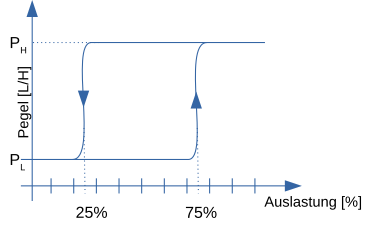
\includegraphics{Hysterese.png}
  \caption{Hysteresekurve der Grenzwerte}
\end{figure}
\pagebreak
\section{Evaluation}

Zur Evaluierung der korrekten Funktion des System, deren Komponenten und Architektur wurde ein eigener Testaufbau entwickelt. Der Testaufbau löst kritische Zustände aus und testet somit den Ablauf des Systems und die kritischen Grenzwerte.

\subsection{Messaufbau}

Für den Messaufbau wurde ein eigener Kubernetes-Service entwickelt, welcher als Pod in das Cluster ausgeliefert wurde. Der Testservice simuliert anormale oder ressourcenintensive Verhaltensweisen und besitzt Funktionen, um die CPU-Last zu maximieren, einen Endpunkt, um die Netzwerkkapazität zu maximieren sowie die Funktion den Arbeitsspeicherbedarf des Service an die kritische Grenze zu bringen.\\
Die Maximierung der CPU-Last erfolgt durch das Berechnen einer rekursiven Funktion, welche die Fibonacci-Zahlenfolge berechnet. Dies hat zur Folge, dass die Last über einen gewissen Zeitraum ansteigt und somit eine Anwendung realitätsnäher Simuliert. Die RAM-Last wird durch das Allokieren von 80\% des Speicherplatzes des Services simuliert. Zum Simulieren der Netzwerklast besitzt der Service einen eigenen HTTP-Post Endpunkt. An diesen Endpunkt wird mittels eines Script dauerhaft und wiederholt ein rund 50 Megabyte großes Script versendet, wodurch die Netzwerklast simuliert wird.\\
Mit diesem Aufbau sollen sowohl die Grenzwerte der Regeln, als auch die Funktion der Komponenten und Architektur als Ganzes und die Anomaliedetection sowie die Ressourcenskalierung getestet werden.
Zum Messen werden Grafen für die CPU-Utilization und RAM-Saturation, den \glqq Replica-Count\grqq sowie den \glqq Rolling-Restart-Count\grqq für jeden Pod und jedes Deployment des Kubernetes-Clusters in der Grafana-Oberfläche erstellt. Der \glqq Rolling-Restart-Count\grqq ist hierbei die Anzahl der Podneustarts für ein Deployment, die mittels \glqq Alert-Action-Manager\grqq ausgeführt wurden. Der \glqq Replica-Count\grqq beschreibt die Anzahl der Pods pro Deployment.

\subsection{Testszenarien}

Es existieren für die Situationen Anomalie und Hochskalieren jeweils drei Szenarien, für das Herunterskalieren eines, womit es sieben zu testende Szenarien gibt.
Diese sind:

\begin{description}
\item[Anomalie]:
\begin{itemize}
\item Hohe CPU-Last, niedrige RAM-Last, niedrige Netzwerklast
\item Niedrige CPU-Last, hohe RAM-Last, niedrige Netzwerklast
\item Hohe CPU- und RAM-Last, niedrige Netzwerklast
\end{itemize}
\item[Hochskalieren]:
\begin{itemize}
\item Hohe CPU-Last, niedrige RAM-Last, hohe Netzwerklast
\item Niedrige CPU-Last, hohe RAM-Last, hohe Netzwerklast
\item Hohe CPU- und RAM-Last, hohe Netzwerklast
\end{itemize}
\item[Herunterskalieren]:
\begin{itemize}
\item Niedrige CPU-Last, niedrige RAM-Last, beliebige Netzwerklast
\end{itemize}
\end{description}

Jedes dieser Szenarien wird in einem eigenen Test evaluiert.
Die maximale Netzlast ist in den Messungen auf den Grenzwert von einem Megabit festgelegt.

\subsection{Messungen}

\subsubsection{Anomalie}

\begin{description}
\item[Hohe CPU-Last, niedrige RAM-Last, niedrige Netzwerklast]:\\

\begin{minipage}{\linewidth}
            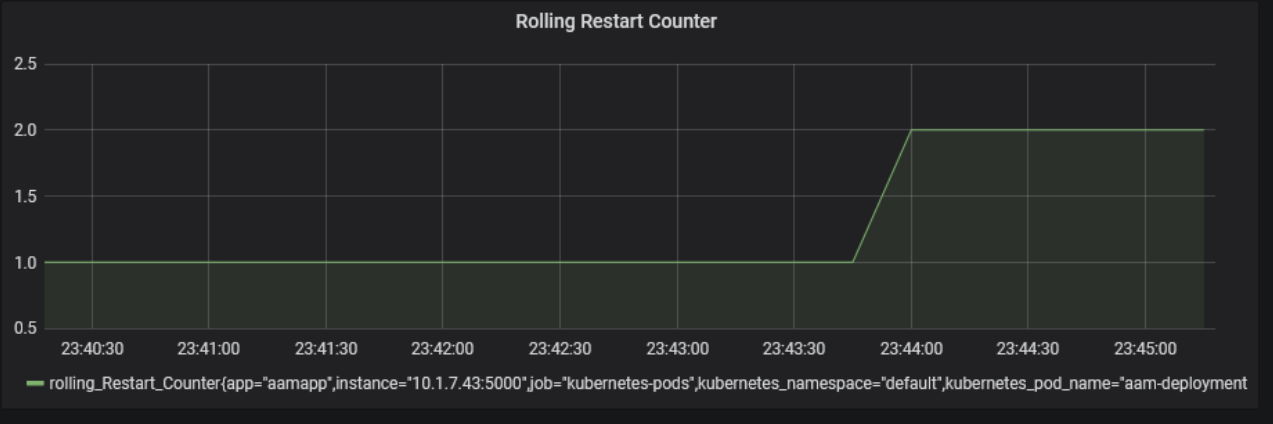
\includegraphics[width=1\textwidth]{img/CPUAnomalie/RollingRestart.PNG}\\
                 
            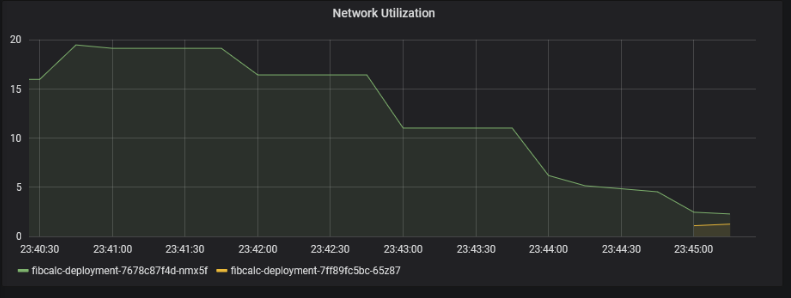
\includegraphics[width=1\textwidth]{img/CPUAnomalie/Netzwerk.PNG}\\
            
            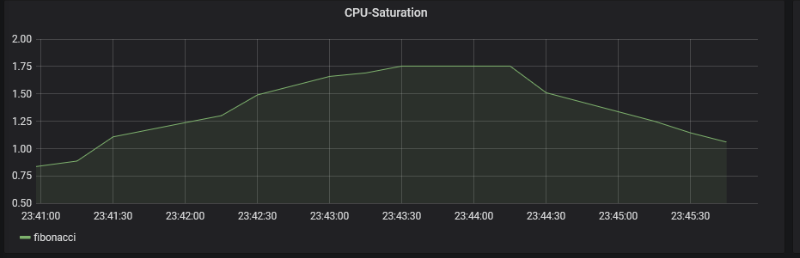
\includegraphics[width=1\textwidth]{img/CPUAnomalie/Saturation.PNG}
\end{minipage}  

\pagebreak
\begin{minipage}{\linewidth}          
  			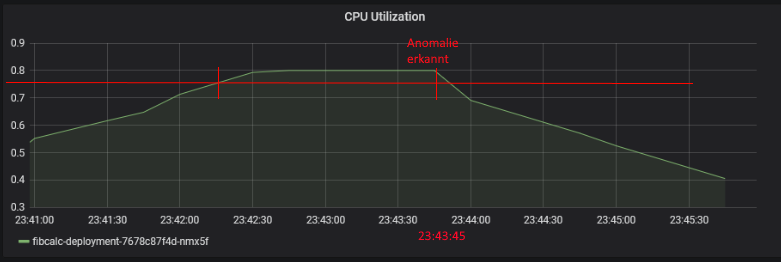
\includegraphics[width=1\textwidth]{img/CPUAnomalie/Utilization.PNG}
            \captionof{figure}{Abbildungen Testwerte Testfall 1 } 
\end{minipage}

Der Zustand eines Pods, bei dem eine hohe CPU-Last von mindestens 75\% besteht, die nicht durch eine Last von außen, das heißt durch eine hohe Netzwerklast, begründet werden kann, ist der Zustand der CPU-Anomalie. Wenn dieser Zustand erreicht ist, soll das System einen \glqq Rolling-Restart\grqq ausführen und somit das anormale Verhalten beenden.\\
Die Graphen zeigen eine stark ansteigende CPU-Last zu Beginn der Messungen. Der CPU Utilization-Graf steigt bis auf eine Last von 80\% an. Diese Höhe hält der Graf eine rund Minute lang, von 23:42:30 bis 23:43:30~45, danach sinkt der Stand des Grafen kontinuierlich ab. Die CPU-Saturation zeigt einen sehr ähnlichen Verlauf mit einem Maximalwert von 175\% Last über eine Minute. Der Graf der Netzwerk-Utilization zeigt einen niedrigen Verlauf bei einem Maximum von 20 Bytes pro Sekunden\\
Der Graf des \glqq Rolling-Restart\grqq -Counter steigt zum Zeitpunkt 23:43:30~45 um eins an.\\
Die Verläufe der Grafen bestätigen, dass die Anomalie korrekt erkannt wurde. Bei einer CPU-Utilization von 80\%, anhaltend über eine Minute und einer niedrigen Netzwerklast von 20 Bytes pro Sekunde, wurde der \glqq Rolling-Restart\grqq durchgeführt, was anhand des ansteigenden \glqq Rolling-Restart\grqq -Counters nachgewiesen wurde. Die CPU-Saturation und Utilization fielen daraufhin erwartungsgemäß ab.

\pagebreak

\item[Niedrige CPU-Last, hohe RAM-Last, niedrige Netzwerklast]:\\

\begin{minipage}{\linewidth}
            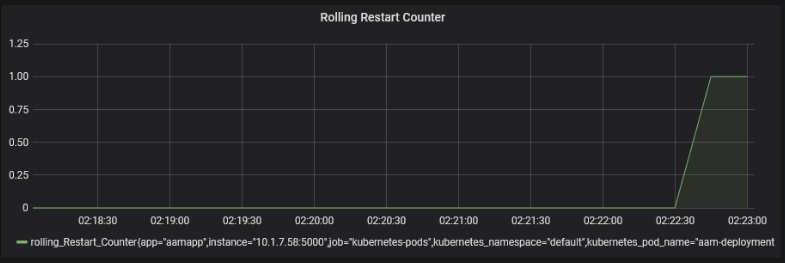
\includegraphics[width=1\textwidth]{img/RAMAnomalie/RollingRestart.PNG}\\
            
            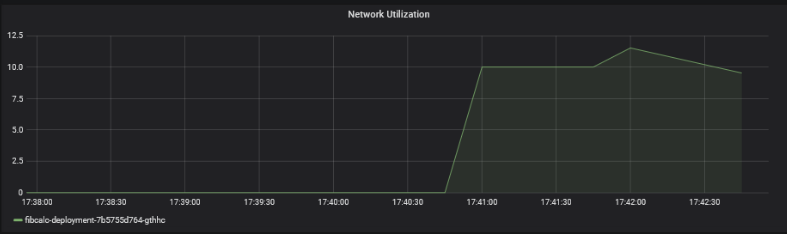
\includegraphics[width=1\textwidth]{img/RAMAnomalie/Netzwerk.PNG}\\
            
            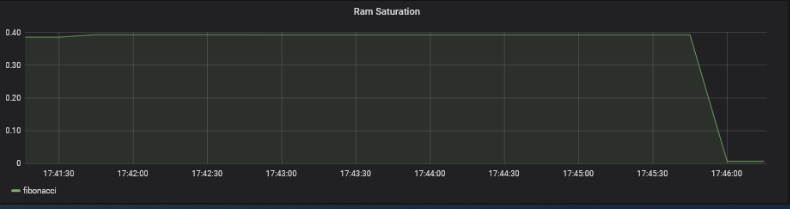
\includegraphics[width=1\textwidth,height=.14\textheight]{img/RAMAnomalie/RAMSaturation.PNG}\\
            
  			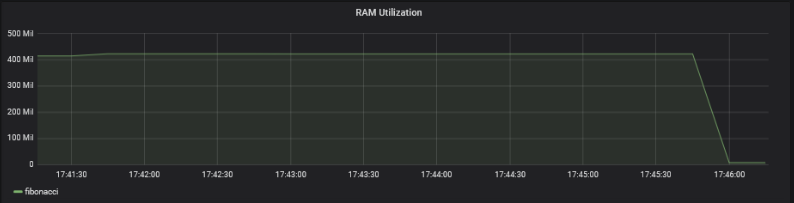
\includegraphics[width=1\textwidth]{img/RAMAnomalie/RAMUtilization.PNG}
            \captionof{figure}{Abbildungen Testwerte Testfall 2}
\end{minipage}

Äquivalent zur CPU-Anomalie wird der Zustand eines Pods als anormal angesehen, wenn eine RAM-Last von mindestens 75\% über den Zeitraum von mindestens einer Minute besteht, die nicht durch eine hohe Netzwerklast begründet wird. Wenn dieser Zustand  der RAM-Anomalie erfüllt ist, soll ein \glqq Rolling-Restart\grqq durchgeführt werden, um die Situation zu entschärfen.\\
Der Graf der RAM-Saturation steigt zwei mal an. Zum Zeitpunkt 02:21:00 auf 75\% und zum Zeitpunkt 02:21:45 bis auf einen Wert von 1,5 an und bricht zwischen den Zeitpunkten 02:22:00 und 02:22:30 ab. Danach ist ein neuer Graf zu erkennen.
Der Verlauf des RAM-Utilization-Grafs steigt bis 800 MByte und verläuft stetig. Ab dem Zeitpunkt 02:22:00 ist, wie bei der Saturation, der Start eines neuen Grafen zu erkennen.
Der Graf der Netzwerk-Utilization zeigt einen niedrigen Verlauf bei einem Maximum von 8 Bytes pro Sekunde.\\
Ab dem Zeitpunkt 02:22:30 ist ein Anstieg um eins bei dem Grafen des \glqq Rolling-Restart\grqq -Counter zu sehen.\\
Die Grafen bestätigen die korrekte Funktion der Anomalieerkennung. Am Graf der RAM-Saturation ist zu erkennen, dass zum Zeitpunkt 02:21:00 der kritische Wert von 75\% RAM-Auslastung erreicht ist. Eine Minute später zum Zeitpunkt 02:22:00 erscheint der neue Pod des Deployments als neuer Graf im Bild, 30 Sekunden später endet der Graf des \glqq alten\grqq Pods. Der Netzwerklast-Graf belegt, dass keine hohe Last von außen auf dem Pod anlag, wodurch ein anormaler Fall vorliegt und der \glqq Rolling-Restart\grqq die korrekte Methode ist.
Der \glqq Rolling-Restart\grqq -Counter wurde um eins nach oben gezählt, was nachweist, dass der Rolling-Restart durchgeführt wurde. 
\pagebreak

\item[Hohe CPU- und RAM-Last, niedrige Netzwerklast]:\\

\begin{minipage}{\linewidth}
            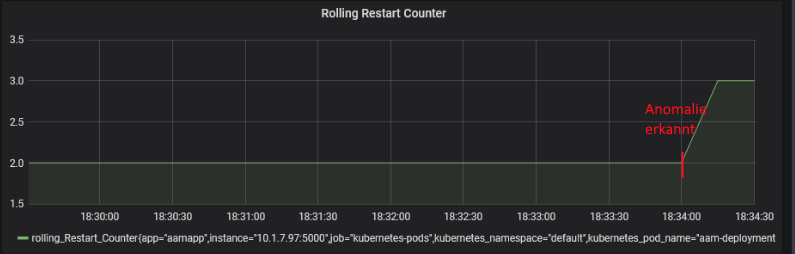
\includegraphics[width=1\textwidth]{img/RAMCPUAnomalie/RollingRestart.PNG}\\
            
            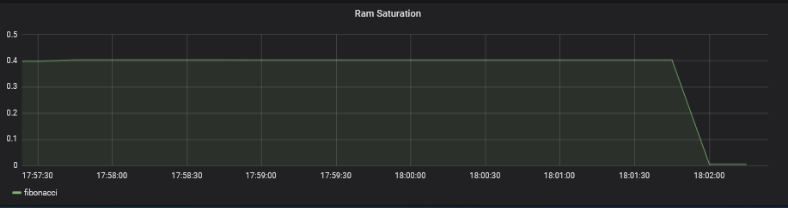
\includegraphics[width=1\textwidth,height=.14\textheight]{img/RAMCPUAnomalie/RAMSaturation.PNG}\\
            
  			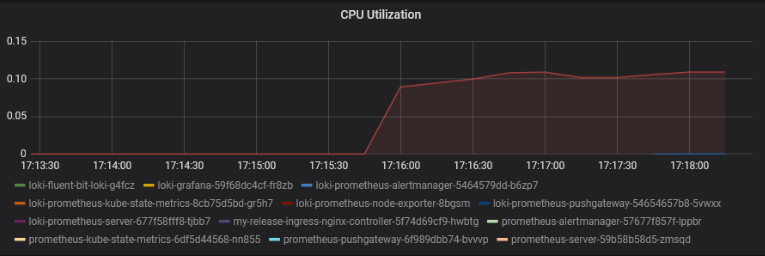
\includegraphics[width=1\textwidth]{img/RAMCPUAnomalie/CPUUtilization.PNG}\\
  			
  			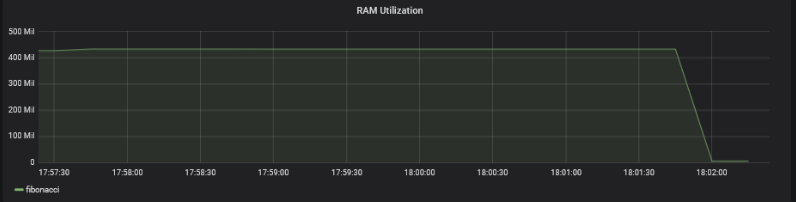
\includegraphics[width=1\textwidth]{img/RAMCPUAnomalie/RAMUtilization.PNG}
\end{minipage}	
\begin{minipage}{\linewidth}	

  			
  			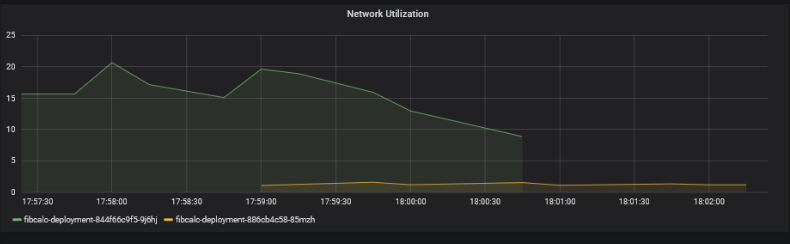
\includegraphics[width=1\textwidth]{img/RAMCPUAnomalie/Netzwerk.PNG}
            \captionof{figure}{Abbildungen Testwerte Testfall 3}
\end{minipage}

Bei einer zeitgleichen Grenzüberschreitung der RAM- und CPU-Utilization und -Saturation von mindestens 75\% liegt ebenfalls ein anormaler Zustand vor. Der Zustand muss eine Minute anhalten und darf auch ebenfalls nur einmal als\\ Anomalie erkannt werden. Der \glqq Rolling-Restart\grqq wird durchgeführt, um die Situation zu entschärfen.\\
Der Graf der CPU-Utilization zeigt von dem Zeitpunkt 18:33:00 bis 18:34:00 einen Wert von über 75\% auf, ab dem Zeitpunkt 18:34:45 ist ein neuer Graf zu erkennen.\\
Der Graf der RAM-Utilization zeigt einen Anstieg auf 800 MByte zum Zeitpunkt 18:32:45. Zur Zeit 18:34:00 erscheint ein neuer, zweiter Graf mit 0\% Last.
Der RAM-Saturation Graf zeigt zum Zeitpunkt 18:32:45 einen Anstieg auf 80\% Last. Zum Zeitpunkt 18:33:45 endet der Graf. Zum Zeitpunkt 18:34:00 erscheint ein neuer, zweiter Graf.
Ab dem Zeitpunkt 18:34:00 ist ein Anstieg um eins bei dem Grafen des \glqq Rolling-Restart\grqq -Counter zu sehen.\\
Der Graf der Netzwerk-Utilization zeigt einen niedrigen Verlauf bei einem Maximum von ~22 Bytes pro Sekunde.\\
Die Grafen belegen die korrekte Funktion und Wirkung der Anomalie-Detection bei hoher RAM- und CPU-Last. Sowohl RAM als auch die CPU haben über den Zeitraum von 18:32:45 ~ 18:33:00 bis 18:34:00 einen Lastwert von über 75\% gehabt. Nach einer Minute wurde ein neuer, zweiter Pod bereitgestellt, was durch den zweiten Grafen zu erkennen ist. Aufgrund der niedrigen Netzlast von 20 Bytes pro Sekunde lag eine anormale Situation vor, weswegen ein \glqq Rolling-Restart\grqq durchzuführen ist. Der \glqq Rolling-Restart-Counter\grqq Graf bestätigt durch das Hochzählen zum Zeitpunkt 18:34:00 die Durchführen dessen. Trotz des Überschreitens zweier Lastwerte wurde wie gewollt nur einmal ein \glqq Rolling-Restart\grqq durchgeführt.

\end{description}

\pagebreak

\subsubsection{Hochskalieren}

\begin{description}

\item[Hohe CPU-Last, niedrige RAM-Last, hohe Netzwerklast]:\\

\begin{minipage}{\linewidth}
            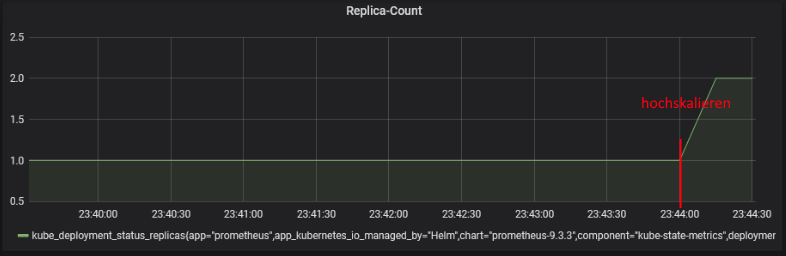
\includegraphics[width=1\textwidth]{img/CPUSkalierung/ReplicaCount.PNG}\\
            
            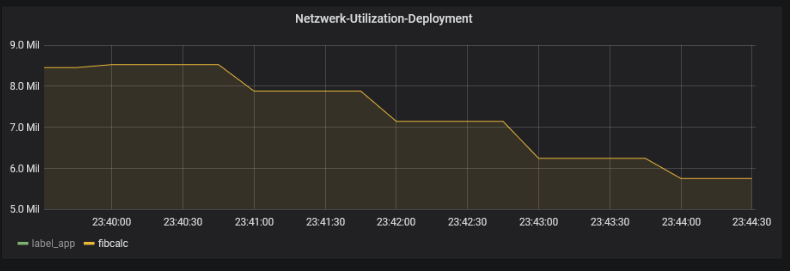
\includegraphics[width=1\textwidth,height=.14\textheight]{img/CPUSkalierung/Netzwerk.PNG}\\
            
  			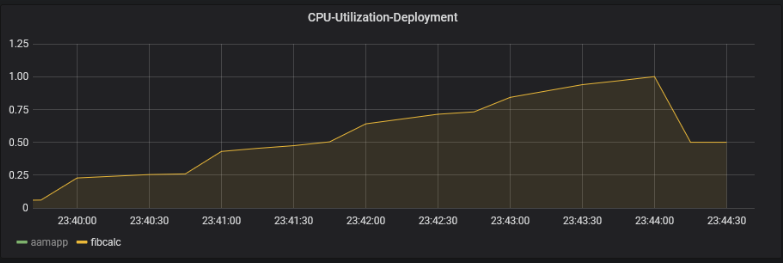
\includegraphics[width=1\textwidth]{img/CPUSkalierung/CPUSaturation.PNG}
            \captionof{figure}{Abbildungen Testwerte Testfall 4}
\end{minipage}

Der Zustand eines Deployments, bei dem eine hohe CPU-Last von mindestens 75\% für den Zeitraum von mindestens einer Minute anliegt, ist der Zustand, in dem Ressourcen hochskaliert werden und somit mehr Ressourcen bereitgestellt werden sollen. Die Ressourcen werden durch das Skalieren der Pods eines Deployments bereitgestellt. Diese Last muss durch eine hohe Netzwerklast von mindestens einem Megabit pro Sekunde von außen begründet werden sein.
Auf dem dargestellten Grafen der CPU-Utilization ist zu sehen, dass der Grenzwert von 75\% zum Zeitpunkt 23:42:45 überschritten wird. Zum Zeitpunkt 23:44:15 sinkt der Graf wieder unter den Grenzwert, auf 50\%. Der Graf des \glqq Replica-Count\grqq zeigt bis zum Zeitpunkt 23:44:00 eine Anzahl von drei an, steigt dann zum Zeitpunkt 23:44:15 auf vier an. Der Graf der Netzwerk zeigt eine durchgehend hohe Last von mindestens rund sechs Megabit.\\
Die Grafen belegen die korrekte Funktion der Skalierung eines Deployments bei hoher CPU-Last. Der CPU-Utilization-Graf zeigt über eine Minute, von Zeitpunkt 23:42:45 bis 23:44:15 eine Utilization von 75\% an, während der Netzwerk-Utilization-Graf eine durchgehende Last über einem Megabit zeigt. Hierdurch wird die Skalierung ausgelöst, was durch den steigenden Wert des \glqq Replica-Count\grqq -Graf zum Zeitpunkt 23:44:15 gezeigt wird. Diese Skalierung bewirkt, dass die CPU-Utilization zur selben Zeit auf einen Wert von 50\% absinkt.

\pagebreak

\item[Niedrige CPU-Last, hohe RAM-Last, hohe Netzwerklast]:\\

\begin{minipage}{\linewidth}
            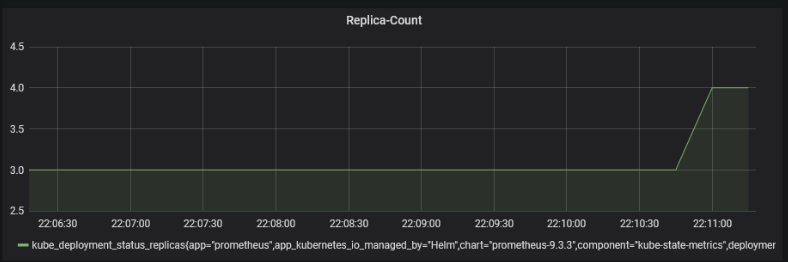
\includegraphics[width=1\textwidth]{img/RAMSkalierung/Replica-Count.PNG}\\
            
            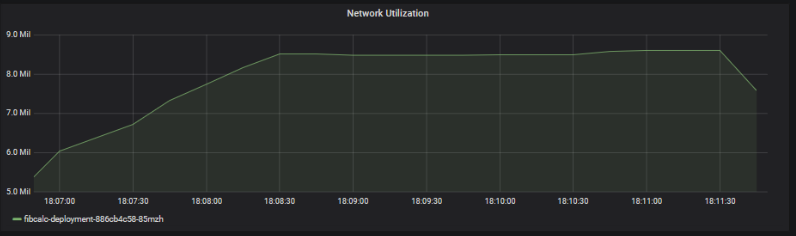
\includegraphics[width=1\textwidth,height=.14\textheight]{img/RAMSkalierung/Netzwerk.PNG}\\
            
  			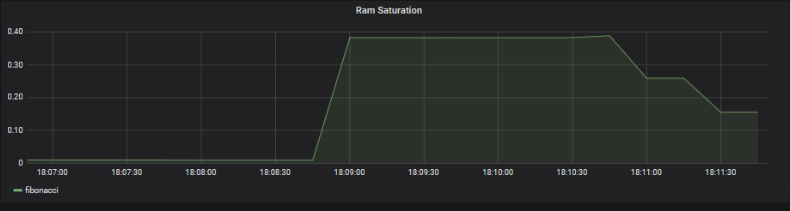
\includegraphics[width=1\textwidth]{img/RAMSkalierung/RAMSaturation.PNG}

            \captionof{figure}{Abbildungen Testwerte Testfall 5}
\end{minipage}

Ein Deployment, dass eine hohe RAM-Last von mindestens 75\% bei einer zeitgleich hohen Netzwerklast von mindestens einem Megabit über den Zeitraum mindestens einer Minute aufweist, benötigt zusätzliche Ressourcen. Diese Ressourcen sollen, wie bei der Skalierung bei hoher CPU-Last auch, durch das Bereitstellen neuer Pods geliefert werden.\\
Auf dem Grafen der RAM-Saturation ist ab dem Zeitpunkt 22:09:00 eine RAM-Saturation von 80\% zu sehen. Ab 22:10:45, fällt diese Last wieder ab unter den Grenzwert auf 60\%. Der Graf der Netzwerklast liegt fast durchgehend bei einem Wert von 3.9 Megabit, mit einem Einbrauch auf einen Wert von 3,3 Megabit. Der \glqq Replica-Counter\grqq -Graf liegt bis zum Zeitpunkt 22:10.45 konstant bei einem Wert von drei, danach steigt er auf den Wert vier an.\\
Die Grafen bestätigen die korrekte Funktion der Skalierung bei hoher RAM-Last. 
Der RAM-Saturation Graf hat über den Zeitraum von über eine Minute einen grenzüberschreitenden Wert von 80\%, während zur selben Zeit die Netzwerklast einen Wert von mindestens 3,3 Megabit und somit einen ausreichend hohen Wert zum Begründen der Last von außen besitzt. In diesem Zustand soll die Skalierung ausgelöst werden, was durch das Ansteigen des \glqq Replica-Counter\grqq -Grafen nachgewiesen wird. Der Wert des Grafen steigt zum Zeitpunkt 22:10:45 von den ursprünglichen drei auf vier, während zum selben Zeitpunkt die RAM-Last des Deployments von 80\% auf ~60\% absinkt, was die Funktion der Skalierung bestätigt.


\pagebreak

\item[Hohe CPU- und RAM-Last, hohe Netzwerklast]:\\

\begin{minipage}{\linewidth}
            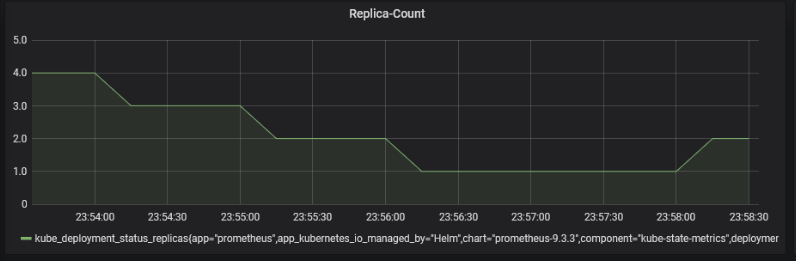
\includegraphics[width=1\textwidth]{img/RAMCPUSkalierung/ReplicaCount.PNG}\\
            
            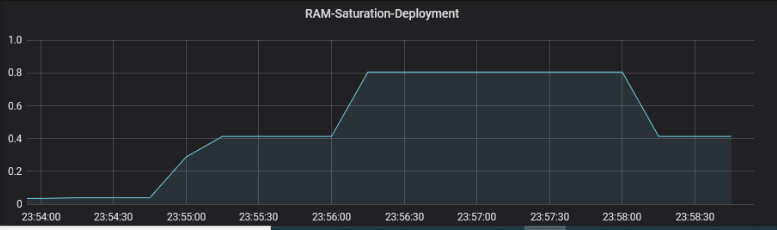
\includegraphics[width=1\textwidth,height=.14\textheight]{img/RAMCPUSkalierung/RAMSaturation.PNG}\\
            
  			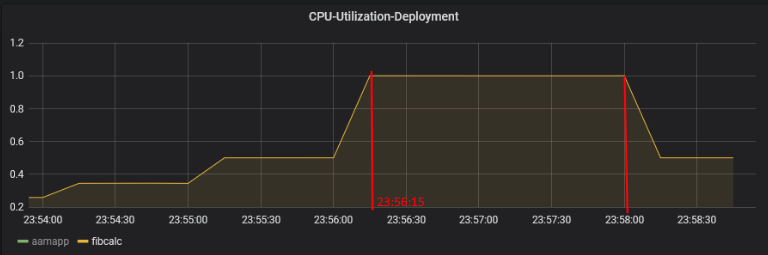
\includegraphics[width=1\textwidth]{img/RAMCPUSkalierung/CPUUtilization.PNG}\\
\end{minipage} 	

\pagebreak

\begin{minipage}{\linewidth}		
  			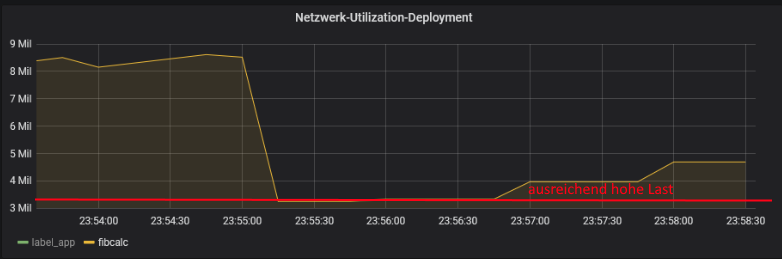
\includegraphics[width=1\textwidth]{img/RAMCPUSkalierung/Netzwerk.PNG}
            \captionof{figure}{Abbildungen Testwerte Testfall 6}
\end{minipage}

Für den Fall, dass CPU- sowie RAM-Last den Grenzwert von 75\% für mindestens eine Minute lang überschreiten, während eine Netzwerklast von mindestens einem Megabit pro Sekunde für das Deployment anliegt, sollen ebenso die Ressourcen des Deployments um einen Pod hochskaliert werden.\\
Die gemessenen Grafen der CPU-Utilization und RAM-Saturation überschreiten beide zum Zeitpunkt 23:56:15 den Grenzwert von 75\% und enden bei einer Last von 80\%. Diese Last hält in beiden Grafen bis zum Zeitpunkt 23:58:00 und \\sinkt danach unter den Grenzwert ab.
Der Graf Netzwerk-Utilization schwankt stark zwischen Werten von drei bis zu neun Megabit pro Sekunde. Der Wert des \glqq Replica-Counter\grqq sinkt anfangs ab, zum Zeitpunkt 23:56:15 hat er den Wert eins. Zum Zeitpunkt 23:58:00 steigt er wieder auf den Wert von zwei an.\\
Die gemessenen Grafen bestätigen, dass die Skalierung auch korrekt funktioniert, wenn gleichzeitig beide Grenzwerte, RAM- sowie CPU-Last, überschritten werden. Beide Werte liegen auf 80\% für mindestens eine Minute mit einer Netzwerk-Utilization von über einem Megabit, bevor die Skalierung durchgeführt wird. Trotz des Überschreitens zweier Werte gleichzeitig, wird nur eine Skalierung durchgeführt. Die Wirkung der Skalierung zeigt sich darin, dass zum Zeitpunkt, zu dem der neue Pod für das Deployment bereitgestellt wurde, die Last beider Werte unter den Grenzwert sinken. Die Durchführung der Skalierung wird durch das Ansteigen des \glqq Replica-Counter\grqq -Grafen um eins dargestellt.

\end{description}

\pagebreak

\subsubsection{Herunterskalieren}

\begin{description}

\item[Niedrige CPU-Last, niedrige RAM-Last, beliebige Netzwerklast]:\\

\begin{minipage}{\linewidth}
            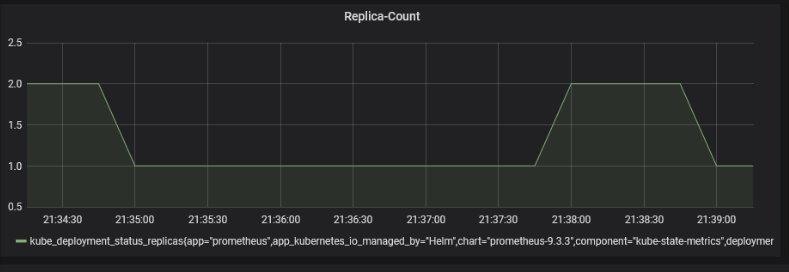
\includegraphics[width=1\textwidth]{img/Herunterskalieren/ReplicaCount.PNG}\\
            
            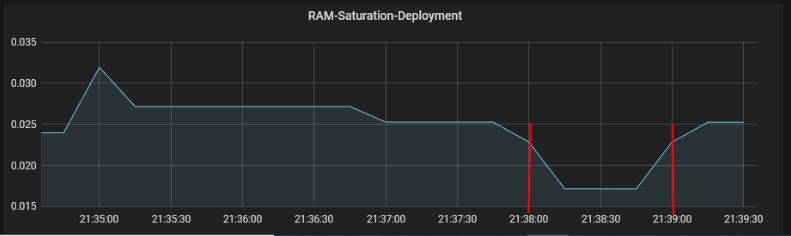
\includegraphics[width=1\textwidth,height=.14\textheight]{img/Herunterskalieren/RAMSaturation.PNG}\\
            
  			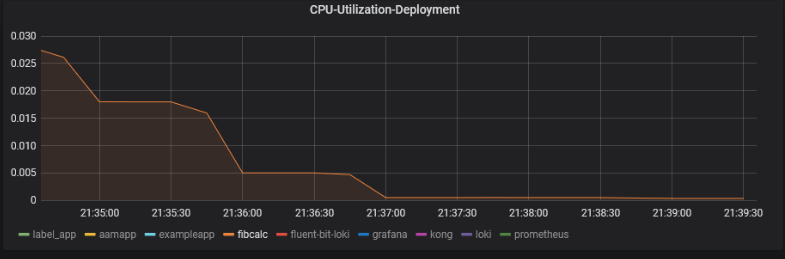
\includegraphics[width=1\textwidth]{img/Herunterskalieren/CPUSaturation.PNG}			
            \captionof{figure}{Abbildungen Testwerte Testfall 7}
\end{minipage}

Im Fall niedriger Ressourcenlast eines Deployments von 25\% CPU-Utilization und RAM-Saturation oder geringer über die Dauer von mindestens einer Minute, soll die Podanzahl des betreffenden Deployments um eins verringert werden.\\
Der Graf der CPU-Utilization zeigt einen absinkenden Verlauf bis zum Zeitpunkt 21:37:00, wo sie ganz auf Null absinkt. Der Graf der RAM-Saturation zeigt einen leicht schwankenden Verlauf. Zum Zeitpunkt 21:37:30 liegt der Wert bei 2,5\% Last, sinkt bei 21:38:00 auf einen Wert von 1,7\% ab, wonach er zum Zeitpunkt 21:39:00 wieder auf den Wert von 2,5\% ansteigt.
Der \glqq Replica-Count\grqq -Graf hat bis zum Zeitpunkt 21:37:30 den Wert eins, steigt dann bei 21:38:00 auf den Wert zwei an und sinkt dann bei 21:39:00 wieder auf eins ab.\\
Der Verlauf der Grafen bestätigt die korrekte Funktion des Herunterskalierens. Die Werte der CPU- sowie RAM-Last liegen beide unter dem Grenzwert von 25\%. Am Grafen des \glqq Replica-Counter\grqq ist zu sehen, dass das Deployment \glqq künstlich\grqq von außen zum Zeitpunkt 21:37:30 auf einen Wert von zwei Pods hochskaliert wurde. Diese Anzahl wurde für eine Minute gehalten und danach zum Zeitpunkt 21:39:00 wieder auf den Wert von einem Pod herunterskaliert.

\end{description}

\pagebreak

\section{Diskussion}

Das Durchführen automatisierter Aktionen auf ein Kubernetes-Cluster ist eine Möglichkeit, Störungsfälle zu reduzieren und unterbrechungsfreie Zeiten zu maximieren. Um diese Automatisierung zu ermöglichen, ist eine Reihe an Tools, Infrastruktur sowie Konfiguration nötig. In dieser Arbeit wurde eine Möglichkeit erarbeitet, diese Automatisierung zu erreichen. Hierfür wurden passende Tools gewählt und entwickelt, mit deren Hilfe sich Daten und Metriken aus einem Kubernetes-Cluster auslesen, darstellen und Aktionen ausführen lassen. Für die gewählten Tools wurde ein System entwickelt, das die korrekte Zusammenarbeit der Tools und Komponenten ermöglicht und koordiniert. Für dieses System wurden Konfiguration sowie ein Regelwerk entworfen und umgesetzt, das Aktionen auf das Cluster definiert und auslöst, die dazu führen, dass auftretende kritische Situationen und Zustände entschärft werden können.\\
In dieser Arbeit konnte gezeigt und evaluiert werden, dass dieses System mithilfe der ausgewählten, quasistandard Monitoring- und Visualisierungskomponenten des \glqq Cloud-Native-Computing\grqq -Bereiches, Prometheus und Grafana, umsetzbar ist, diese aber durch weitere Komponenten ergänzt werden müssen. Daher wurde im Rahmen der Arbeit das Tool \glqq Alert-Action-Manager\grqq entwickelt, das die fehlenden Funktionen ergänzt, die das Ableiten von Aktionen aus Alerts von Prometheus ermöglicht. \\
In der folgenden Diskussion wird die Evaluation, der Rahmen des Projekts, aufgetretene Probleme und mögliche Verbesserungen in der Zukunft des Projekts diskutiert.

\subsection{Rahmen des Projekts}

Der Rahmen dieses Projekts beinhaltet die Wahl geeigneter Tools zur Umsetzung an einem bereits bestehenden Kubernetes-Cluster, die Entwicklung der geeigneten Systemarchitektur mithilfe dieser Tools und die Konfiguration, die nötig ist, um diese funktionsfähig zumachen.
Neben den in diesem Projekt eingesetzten, von der \glqq Cloud-Native-Computing-Foundation\grqq empfohlenen Tools, Prometheus und Grafana, gibt es noch weitere Tools, mit denen sich dieses Projekt hätte realisieren lassen können, wie beispielsweise die Tool-Sammlung \glqq ELK\grqq -Stack. Aufgrund des zeitlichen Rahmens und bereits vorhandenen Erfahrungen auf dem Gebiet der Tools Prometheus und Grafana zu Projektbeginn, wurde eine weitere Toolauswahl nicht durchgeführt.

\subsection{Evaluation}

In der Evaluation wurde die Funktion des Gesamtsystem getestet und mithilfe von aufgezeichneten Grafen gemessen. Hierbei konnte für alle Testfälle die korrekte Funktion in angemessener Zeit nachgewiesen werden.\\
Die Evaluation ergab indes auch, dass Aktionen teilweise mit einer Verzögerung und Messungenauigkeiten von einigen Sekunden ausgeführt werden, sichtbar beispielsweise im Graf des Testfalls \glqq Hohe CPU- und RAM-Last, hohe Netzwerklast\grqq , bei dem die Skalierung erst deutlich nach einer Minute eintritt. Im Rahmen dieses Projekts ist diese Verzögerung vertretbar, da die durchgeführten Aktionen der Skalierung und Anomaliedetektion nicht sekundenkritisch sind und auch mit einigen Sekunden Verzögerung ausgeführt, immer noch ihren Zweck erfüllen. Für sekundenkritische Aktionen wäre das System dieser Arbeit aufgrund der Verzögerungen aber unter Umständen nicht geeignet.\\

\subsection{Probleme}

Während der Bearbeitung sind einige Probleme entstanden, die in diesem Projekt behoben werden konnten, für andere Aktionen in Zukunft möglicherweise aber Probleme darstellen könnten und mögliche Grenzen des eingesetzten Systems aufzeigen:\\

\begin{description}

\item[Zu viele versendete Alert-Nachrichten]:\\

Prometheus bzw. der Prometheus-Alertmanager versendet Alert-Nachrichten sobald eine Alertregel erfüllt ist. Bei dem Versenden der Alerts kann es dazu kommen, dass diese mehrfach versendet werden. Da das Ausführen der Aktionen im \glqq Alert-Action-Manager\grqq auf dem Erhalt der Alert-Nachrichten basiert, wird eine Aktion teils mehrfach für einen Alert ausgeführt. Dieses Problem musste programmatisch abgefangen werden, indem eingegangene Nachrichten anhand ihrer Versendezeit gespeichert werden.

\item[Zeittoleranzen]:\\

Wie bei der Evaluation bereits erläutert, können Messungenauigkeiten und Toleranzen dazu führen, dass sich Zeiträume, in welchen die Aktionen ausgeführt werden, erhöhen. Zusätzlich kommen noch mögliche Verzögerungen durch das Versenden und durch die Ausführung der Aktionen hinzu.

\item[Statische Grenzwerte und Regeln]:\\

Das System basiert auf statisch konfigurierten Regeln mit festen Grenzwerten. Kubernetes-Cluster, die sich in ständiger Entwicklung befinden und deren verfügbare Ressourcen sich verändern, bedürfen einer nachträglichen Konfiguration der Regeln und Grenzwerte. Bei einer großen Anzahl von konfigurierten Regeln kann dies zu hohem Aufwand durch Konfiguration und Tests sowie erhöhter Fehleranfälligkeit führen.

\end{description}
 
\subsection{Zukunft des Projekts}

Das in dieser Arbeit bearbeitete Projekt bildet die Grundlage für ein System, das Aktionen aufgrund von Zuständen in einem Cluster ausführen kann. Dieses System kann neben den in diesem Projekt eingesetzten Aktionen Anomaliedetektion und Skalierung um beliebige weitere Aktionen erweitert werden.\\
Des Weiteren kann es, um den erläuterten Problemen dieses Systems entgegenzuwirken, eine Lösung sein, ein anderes Monitoringsystem mit ähnlichen Eigenschaften und Funktionen wie das regelbasierte Alerting von Prometheus, zu testen.\\
Sofern dieses Projekt für ein dynamischeres und größeres System in Zukunft eingesetzt werden soll, kann der Ansatz der statischen Regel durch einen \glqq Machine-Learning\grqq -basierten Ansatz, wie im Kapitel drei \glqq Stand der Technik\grqq vorgestellt, ergänzt oder ersetzt werden.

\section{Fazit und Ausblick}

Zusammenfassend kann über dieses Projekt gesagt werden, dass es erfolgreich beendet werden konnte. In dieser Arbeit wurde ein möglicher Weg entwickelt, der regelbasiert automatisierte Aktionen wie die Anomaliedetection oder die Skalierung auf ein Kubernetes-Cluster ausführt. Ebenso wurden auch mögliche Probleme, wie hohe Zeittoleranzen, in diesem Systems erkannt, welche es für einige zeitkritische Anwendungszwecke unbrauchbar machen könnten.\\
Trotzdem stellt dieser Ansatz vor allem einen sehr leichtgewichtigen und im Gegensatz zu den vorgestellten, Machine-Learning-basierten Ansätzen einen einfacher nachvollziehbaren und deterministischeren Ansatz dar.\\
Dieses Projekt wird in der Zeit nach dieser Arbeit weiter betrieben und Teil einer produktiven Infrastruktur werden. Zu diesem Zeitpunkt geplante Erweiterungen sind weitere Regeln sowie der Einsatz der kuberneteseigenen Skalierungsfunktion \glqq HPA\grqq.

\newpage
\bibliography{Literatur}

\newpage


\end{document}